%
% Main document
% ===========================================================================
% This is part of the document "Project documentation template".
% Authors: brd3, kaa1
%
%---------------------------------------------------------------------------
\documentclass[
    a4paper,                    % paper format
    10pt,                           % fontsize
    %twoside,                    % double-sided
    openright,              % begin new chapter on right side
    notitlepage,            % use no standard title page
    parskip=half,           % set paragraph skip to half of a line
]{scrreprt}                 % KOMA-script report
%---------------------------------------------------------------------------
\raggedbottom{}
%\KOMAoptions{cleardoublepage=plain}         % Add header and footer on blank pages


% Load Standard Packages:
%---------------------------------------------------------------------------
\usepackage{scrpage2}
\usepackage[standard-baselineskips]{cmbright}
\usepackage[ngerman]{babel}                                             % german hyphenation
\usepackage[utf8]{inputenc}                                             % UTF-8 input encoding
\usepackage[T1]{fontenc}                                                % hyphenation of words with ä,ö and ü
\usepackage{textcomp}                                                   % additional symbols
\usepackage{etoolbox}                                                   % color manipulation of header and footer
\usepackage{graphicx}                                                   % integration of images
\usepackage{float}                                                      % floating objects
\usepackage[font={footnotesize,it}]{caption}                                                    % for captions of figures and tables
\usepackage{booktabs}                                                   % package for nicer tables
\usepackage{tocvsec2}                                                   % provides means of controlling the sectional numbering
\usepackage[square,sort,comma,numbers]{natbib}                           % provides various citation styles
\usepackage{wrapfig}                                                    % provides floating of text around images
\usepackage{nameref}                                                    % provides printing names of references
\usepackage{colortbl}                                                   % Colored tables
\usepackage{scrhack}                                                    % Remove float errors and warnings
\usepackage{pgfgantt}                                                   % Provides GANTT charts
%---------------------------------------------------------------------------

% Load Math Packages
%---------------------------------------------------------------------------
\usepackage{amsmath}                                                    % various features to facilitate writing math formulas
\usepackage{amsthm}                                                     % enhanced version of latex's newtheorem
\usepackage{amsfonts}                                                   % set of miscellaneous TeX fonts that augment the standard CM
\usepackage{amssymb}                                                    % mathematical special characters
\usepackage{exscale}                                                    % mathematical size corresponds to textsize
%---------------------------------------------------------------------------

% Package to facilitate placement of boxes at absolute positions
%---------------------------------------------------------------------------
\usepackage[absolute]{textpos}
\setlength{\TPHorizModule}{1mm}
\setlength{\TPVertModule}{1mm}
%---------------------------------------------------------------------------                    

% Definition of Colors
%---------------------------------------------------------------------------
\RequirePackage{color}                          % Color (not xcolor!)
\definecolor{linkblue}{rgb}{0,0,0.8}            % Standard
\definecolor{darkblue}{rgb}{0,0.08,0.45}        % Dark blue
\definecolor{bfhgrey}{rgb}{0.41,0.49,0.57}      % BFH grey
%\definecolor{linkcolor}{rgb}{0,0,0.8}              % Blue for the web- and cd-version!
\definecolor{linkcolor}{rgb}{0,0,0}                 % Black for the print-version!

%---------------------------------------------------------------------------

% Load listings package
% which provides source code formatting
%---------------------------------------------------------------------------
\usepackage{listings}                                                   % provides source code formatting
% Define XML colors
\lstdefinelanguage{XML}
{
  basicstyle=\ttfamily\footnotesize,
  morestring=[b]'',
  moredelim=[s][\bfseries\color{maroon}]{<}{\ },
  moredelim=[s][\bfseries\color{maroon}]{</}{>},
  moredelim=[l][\bfseries\color{maroon}]{/>},
  moredelim=[l][\bfseries\color{maroon}]{>},
  morecomment=[s]{<?}{?>},
  morecomment=[s]{<!--}{-->},
  commentstyle=\color{codecommentcolor},
  stringstyle=\color{darkblue},
  identifierstyle=\color{red}
}

%---------------------------------------------------------------------------

% Hyperref Package (Create links in a pdf)
%---------------------------------------------------------------------------
\usepackage[
    pdftex,ngerman,bookmarks,plainpages=false,pdfpagelabels,
    backref = {false},                                      % No index backreference
    colorlinks = {true},                  % Color links in a PDF
    hypertexnames = {true},               % no failures "same page(i)"
    bookmarksopen = {true},               % opens the bar on the left side
    bookmarksopenlevel = {0},             % depth of opened bookmarks
    pdftitle = {Template für Bachelor Thesis},      % PDF-property
    pdfauthor = {brd3},                           % PDF-property
    pdfsubject = {LaTeX Template},        % PDF-property
    linkcolor = {linkcolor},              % Color of Links
    citecolor = {linkcolor},              % Color of Cite-Links
    urlcolor = {linkcolor},               % Color of URLs
]{hyperref}
%---------------------------------------------------------------------------
% Set up page dimension
%---------------------------------------------------------------------------
\usepackage{geometry}
\geometry{a4paper,
    left=28mm,
    right=15mm,
    top=30mm,
    headheight=20mm,
    headsep=10mm,
    textheight=242mm,
    footskip=15mm
}
%---------------------------------------------------------------------------

% Makeindex Package
%---------------------------------------------------------------------------
\usepackage{makeidx}                                % To produce index
\makeindex                                      % Index-Initialisation
%---------------------------------------------------------------------------

% Glossary Package
%---------------------------------------------------------------------------
% the glossaries package uses makeindex
% if you use TeXnicCenter do the following steps:
%  - Goto "Ausgabeprofile definieren" (ctrl + F7)
%  - Select the profile "LaTeX => PDF"
%  - Add in register "Nachbearbeitung" a new "Postprozessoren" point named Glossar
%  - Select makeindex.exe in the field "Anwendung" ( ..\MiKTeX x.x\miktex\bin\makeindex.exe )
%  - Add this [ -s "%tm.ist" -t "%tm.glg" -o "%tm.gls" "%tm.glo" ] in the field "Argumente"
%
% for futher informations go to http://ewus.de/tipp-1029.html
%---------------------------------------------------------------------------
\usepackage[nonumberlist]{glossaries}
%\usepackage[xindy,nonumberlist]{glossaries}

% das zügs do unde dra find i eigendli unnötig, wenn mir so afön fülle mir sitewiss mit "`unüebliche"' begriffe! :(
\newglossaryentry{UML}{name={Wissensmodellierung},description={...}}
\newglossaryentry{Relationale Datenbank}{name={Beschreibungslogik },description={Reasoner ...}}
\newglossaryentry{Relationale Datenspeicherung}{name={Beschreibungslogik },description={Reasoner ...}}
\newglossaryentry{Semantische Datenbank}{name={Beschreibungslogik },description={Reasoner ...}}
\newglossaryentry{Expertensystem}{name={Beschreibungslogik },description={Reasoner ...}}
\newglossaryentry{Ontologie}{name={Ontologie},description={...}}
\newglossaryentry{Domäne}{name={Beschreibungslogik },description={Reasoner ...}}
\newglossaryentry{Wissensdomäne}{name={Beschreibungslogik },description={Reasoner ...}}
\newglossaryentry{Problemdomäne}{name={Beschreibungslogik },description={Reasoner ...}}
\newglossaryentry{Reasoner}{name={Beschreibungslogik },description={Reasoner ...}}
\newglossaryentry{Inferenzmaschine}{name={Beschreibungslogik },description={Reasoner ...}}
\newglossaryentry{Tutorial}{name={Beschreibungslogik },description={Reasoner ...}}
\newglossaryentry{RDF/XML}{name={Resolution},description={...}}
\newglossaryentry{OWL/XML}{name={Parser },description={...}}

\newglossaryentry{Semantik}{name={Inferenz},description={...}}
\newglossaryentry{Knowledge-Engineering}{name={Wissensmodellierung},description={...}}
\newglossaryentry{Knowledge-Engineer}{name={Wissensingeneur},description={Analytiker, Informationsmanager mit entsprechender Methodik und entsprechenden Werkzeugen}}
\newglossaryentry{HERMES}{name={Resolution},description={...}}
\newglossaryentry{Scrum}{name={Inferenz},description={...}}
\newglossaryentry{RDF}{name={Resolution},description={...}}
\newglossaryentry{OWL}{name={Inferenz},description={...}}
\newglossaryentry{Ontologie-Sprache}{name={Inferenz},description={...}}
\newglossaryentry{SWRL}{name={Inferenz},description={...}}
\newglossaryentry{SPARQL}{name={Inferenz},description={...}}
\newglossaryentry{W3C}{name={Inferenz},description={...}}
\newglossaryentry{Apache Stanbol}{name={Inferenz},description={...}}
\newglossaryentry{Stanford Protégé}{name={Inferenz},description={...}}
\newglossaryentry{Clark & Parsia Stardog}{name={Inferenz},description={...}}
\newglossaryentry{XML}{name={Inferenz},description={...}}
\newglossaryentry{Graphdatenbank}{name={Beschreibungslogik },description={Reasoner ...}}
\newglossaryentry{yWorks yEd}{name={Beschreibungslogik },description={Reasoner ...}}
\newglossaryentry{Unifikation}{name={Beschreibungslogik },description={Reasoner ...}}
\newglossaryentry{Semantisches Netz}{name={Parser },description={...}}
\newglossaryentry{NP-vollständig}{name={Parser },description={...}}
\newglossaryentry{URL}{name={Parser },description={...}}
\newglossaryentry{Turtle}{name={Parser },description={...}}
\newglossaryentry{FACT++}{name={Parser },description={...}}
\newglossaryentry{Pellet}{name={Beschreibungslogik },description={Reasoner ...}}
\newglossaryentry{SNARL}{name={Beschreibungslogik },description={Reasoner ...}}
%bis 6.2.1 ok
\newglossaryentry{Resolution}{name={Resolution},description={...}}
\newglossaryentry{Inferenz}{name={Inferenz},description={...}}

\newglossaryentry{Wissensakquise}{name={Wissensakquise},description={Sammeln/ erfassen, aufarbeiten/strukturieren von Wissen}}
\newglossaryentry{Parser}{name={Parser },description={...}}

\newglossaryentry{Beschreibungslogik}{name={Beschreibungslogik },description={Reasoner ...}}
\newglossaryentry{Frame}{name={Parser },description={...}}
\newglossaryentry{Wissensnetzte }{name={Parser },description={...}}

\newglossaryentry{Konzepte}{name={Parser },description={...}}
\newglossaryentry{Axiome}{name={Parser },description={...}}
\newglossaryentry{Prinzipien}{name={Parser },description={...}}
\newglossaryentry{Wissensmodellierung}{name={Beschreibungslogik },description={Reasoner ...}}

\newglossaryentry{Semantisches Web}{name={Beschreibungslogik },description={Reasoner ...}}
\newglossaryentry{Semantik}{name={Beschreibungslogik },description={Reasoner ...}}
\newglossaryentry{Formale Sprache}{name={Beschreibungslogik },description={Reasoner ...}}
\newglossaryentry{Künstliche Intelligenz}{name={Beschreibungslogik },description={Reasoner ...}}
\newglossaryentry{Aussagenlogik}{name={Beschreibungslogik },description={Reasoner ...}}
\newglossaryentry{Prädikatenlogik}{name={Beschreibungslogik },description={Reasoner ...}}

\newglossaryentry{Hierarchische Datenbank}{name={Beschreibungslogik },description={Reasoner ...}}
%\newglossaryentry{Graph}{name={Beschreibungslogik },description={Reasoner ...}}
%\newglossaryentry{Zyklenfreie Nachbarschaft}{name={Beschreibungslogik },description={Reasoner ...}}
%\newglossaryentry{Entität}{name={Beschreibungslogik },description={Reasoner ...}}
%\newglossaryentry{Knoten}{name={Beschreibungslogik },description={Reasoner ...}}
%\newglossaryentry{Kanten}{name={Beschreibungslogik },description={Reasoner ...}}
\newglossaryentry{Existenzaussage}{name={Beschreibungslogik },description={Reasoner ...}}
\newglossaryentry{Ontologiesprache}{name={Beschreibungslogik },description={Reasoner ...}}

\newglossaryentry{Modus Ponens}{name={Beschreibungslogik },description={Reasoner ...}}
\newglossaryentry{Theorem}{name={Beschreibungslogik },description={Reasoner ...}}

\newglossaryentry{Tableau-Kalkül}{name={Beschreibungslogik },description={Reasoner ...}}
\newglossaryentry{Prämisse}{name={Beschreibungslogik },description={Reasoner ...}}
\newglossaryentry{Konklusion}{name={Beschreibungslogik },description={Reasoner ...}}
\newglossaryentry{Literal}{name={Beschreibungslogik },description={Reasoner ...}}
\newglossaryentry{xxx}{name={Beschreibungslogik },description={Reasoner ...}}


\makeglossaries{}
%---------------------------------------------------------------------------

% Intro:
%---------------------------------------------------------------------------
%\begin{document}                                % Start Document
\settocdepth{section}                                                       % Set depth of toc
\pagenumbering{roman}                                                       
%---------------------------------------------------------------------------

\providecommand{\titel}{Titel des Berichts}		%  Hier den Titel des Berichts/Thesis eingeben                  % Titel der Arbeit aus Datei titel.tex lesen
\providecommand{\versionnumber}{0.1}			%  Hier die aktuelle Versionsnummer eingeben
\providecommand{\versiondate}{08.06.2014}		%  Hier das Datum der aktuellen Version eingeben
                % Versionsnummer und -datum aus Datei version.tex lesen

% Set up header and footer
%---------------------------------------------------------------------------

\deftripstyle{newlayout}
  [0pt] % no header line
  [0pt] % no footer line
  {}
  {}
  {}
  {\color{bfhgrey} \footnotesize \titel, Version \versionnumber, \versiondate}
  {}
  {\color{bfhgrey} \thepage}

\pagestyle{newlayout}
% use "pagestyle" also on chapter starting pages 
\renewcommand{\chapterpagestyle}{newlayout}
\renewcommand{\chaptermark}[1]{\markboth{\thechapter.  #1}{}}
\renewcommand*{\headfont}{\normalfont}
\renewcommand*{\footfont}{\normalfont}
%---------------------------------------------------------------------------

% We need this as mr. gantt chart (teh package..) thinks text should be gray..
\color{black}

\begin{document}

% Title Page and Abstract
%---------------------------------------------------------------------------
%
% Project documentation template
% ===========================================================================
% This is part of the document "Project documentation template".
% Authors: brd3, kaa1
%

\begin{titlepage}


% BFH-Logo absolute placed at (28,12) on A4 and picture (16:9 or 15cm x 8.5cm)
% Actually not a realy satisfactory solution but working.
%---------------------------------------------------------------------------
\setlength{\unitlength}{1mm}
\begin{textblock}{20}[0,0](28,12)
    
\includegraphics[scale=1.0]{bilder/BFH_Logo_B.png}
\end{textblock}

\begin{textblock}{154}(28,48)
    \begin{picture}(150,2)
        \put(0,0){\color{bfhgrey}\rule{150mm}{2mm}}
    \end{picture}
\end{textblock}

\begin{textblock}{154}[0,-0.2](28,42)
    \centering
    
\includegraphics[scale=0.7]{bilder/owl.png}   % Titelbild definieren
\end{textblock}

\begin{textblock}{154} (28,135)
    \begin{picture}(150,2)
        \put(0,0){\color{bfhgrey}\rule{150mm}{2mm}}
    \end{picture}
\end{textblock}
\color{black}

% Institution / Titel / Untertitel / Autoren / Experten:
%---------------------------------------------------------------------------
\begin{flushleft}

\vspace*{120mm}

\fontsize{26pt}{28pt}\selectfont
\titel% Titel aus der Datei vorspann/titel.tex lesen
\vspace{3mm}



\fontsize{10pt}{12pt}\selectfont
\textbf{Aufbau von Wissensdomänen anhand einer semantischen Datenbank} \\                                 % eingeben
\vspace{3mm}

\begin{textblock}{150} (28,215)
\fontsize{10pt}{17pt}\selectfont
\begin{tabbing}
xxxxxxxxxxxxxxx\=xxxxxxxxxxxxxxxxxxxxxxxxxxxxxxxxxxxxxxxxxxxxxxx \kill
Autoren:        \> Sven Osterwalder, Mira Günzburger     \\                  % Namen eingeben
Datum:          \> \versiondate\\      % aus Datei vorspann/version.tex lesen
\end{tabbing}

\end{textblock}
\end{flushleft}

\begin{textblock}{150} (28,280)
\noindent 
\color{bfhgrey}\fontsize{9pt}{10pt}\selectfont
Berner Fachhochschule | Haute école spécialisée bernoise | Bern University of Applied Sciences
\color{black}\selectfont
\end{textblock}


\end{titlepage}

%
% ===========================================================================
% EOF
%
          % activate for Titelseite mit Bild
\cleardoublepage{}
\phantomsection{}
% Versionenkontrolle :
% -----------------------------------------------

\begin{textblock}{180} (15,150)
\color{black}
\begin{huge}
Versionen
\end{huge}
\vspace{10mm}

\fontsize{10pt}{18pt}\selectfont
\begin{tabbing}
xxxxxxxxxxx\=xxxxxxxxxxxxxxx\=xxxxxxxxxxxxxx\=xxxxxxxxxxxxxxxxxxxxxxxxxxxxxxxxxxxxxxxxxxxxxxx \kill
Version	\> Datum	\> Status		\> Bemerkungen		\\
0.1	\> 08.06.2014	\> Entwurf		\> Anforderungsdokument erstellen	\\	
0.2	\> 08.08.2014	\> Entwurf		\> Korrekturen und Ergänzungen	\\	
0.3	\> 19.09.2014	\> Entwurf		\> Anpassungen an die Aufgabenstellung	\\ 
%0.3	\> 02.09.2013	\> Entwurf		\> Donec eget aliquam urna. Lorem ipsum dolor sit amet	\\ 
%1.0	\> 12.09.2013	\> Definitiv	\> Lorem ipsum dolor sit ametPhasellus scelerisque, leo sed iaculis ornare 	\\ 
%1.1	\> 04.11.2013	\> Korrektur	\> Layout angepasst	\\
\end{tabbing}

\end{textblock}

\phantomsection{}
\cleardoubleemptypage{}
\setcounter{page}{1}
\cleardoublepage{}
\phantomsection{}
\cleardoubleemptypage{}
%---------------------------------------------------------------------------

% Make sure Umlauts are getting displayed correctly.
\lstset{literate=%
    {Ö}{\textcolor{red}{\"O}}1
    {Ä}{{\"A}}1
    {Ü}{{\"U}}1
    {ß}{{\ss}}1
    {ü}{{\"u}}1
    {ä}{{\textcolor{red}{\"a}}}1
    {ö}{{\textcolor{red}{\"o}}}1
    {~}{{\textasciitilde}}1
    {?}{{\textcolor{red}{?}}}1
}

% Table of contents
%---------------------------------------------------------------------------
\tableofcontents
\cleardoublepage{}
%---------------------------------------------------------------------------

% Main part:
%---------------------------------------------------------------------------
\pagenumbering{arabic}
\chapter{Einleitung}
\label{chap:einleitung}

%CHeckliste fausibibel
%Ausgangslage, Problemstellung
%• Auftrag oder Aufgabenstellung
%• Resultat der Arbeit
%• Methodik (Herkunft der Daten, Vorgehen, Systemund
%Gültigkeitsgrenzen)
%• Folgerungen, offene Fragen

Der klassische Ansatz der Wissensabbildung, zum Beispiel in Form von UML, welchem die relationale Datenspeicherung zugrunde liegt, wird in der heutigen Informatik weitläufig eingesetzt und ist de facto Standard. Häufig geschieht dies in enger Verbindung mit der objektorientierten Programmierung. Experten aus einer Fachrichtung sind fähig diese Daten zu interpretieren und daraus Schlüsse zu ziehen. Es ist aber nicht möglich automatisch Fragestellungen zu beantworten, welche über reine Relationsverknüpfungen hinausgehen. Mit dieser Technik sind Objekteigenschaften und -Verhalten also eher schwer abbildbar. Eine andere Art Wissen zu repräsentieren sind semantische Datenbanken. Diese ermöglichen das Abbilden des Objektverhaltens und können mithilfe von Schlussfolgerungen die Rolle des Experten einnehmen.

In dieser Bachelorthesis soll eine solche semantische Datenbank aufgebaut und angewendet werden.  Die Arbeit wurde in zwei Teilen umgesetzt: Einem  theoretischen und einem praktischen Teil. Der theoretische Teil zeigt in Form eines Tutorials auf, wie ein knowledge engineer bei der Wissensmodellierung vorgeht. Er nutzt dabei Ontologien als Basis, um eine semantische Datenbank aufzubauen. Im praktischen Teil soll eine solche Ontologie aufgebaut und per Benutzerschnittstelle zugänglich gemacht werden.

Die gesteckten Ziele konnten allesamt erreicht werden. Es ist den Autoren gelungen die Theorie der Wissensmodellierung übersichtlich in einem Dokument aufzubereiten und wiederzugeben. Speziell dabei ist, dass in diesem fachliche Grundlagen mit einem praktischen Beispiel verbunden werden. Zusätzlich konnten auch konkrete Tipps aus der eigenen Erfahrung eingeflochten werden. Dieses Dokument ist dem Abschlussdokument als Anhang beigefügt.

Im praktischen Teil der Arbeit wurde ein Expertensystem für Reisen aufgebaut: ``In der heutigen Zeit werden Ferien häufig per Internet gebucht. Was aber, wenn der Urlaub nicht einfach zwei Wochen an einem Ort stattfinden soll? Was, wenn der Kunde reisen möchte? Oder sonstige spezielle Wünsche hat? Für solche Anforderungen muss er auch heute noch in ein Reisebüro um sich beraten zu lassen.''\\
Bei der Automatisierung dieses Prozesses kommt die Ontologie ins Spiel, welche mithilfe von Eigenschaften, Kriterien und Regeln die Problemdomäne abbildet. Durch die Verwendung eines Reasoners können verschiedene Reisevorschläge gemacht werden.\\
Um eine sehr individuelle Reiseplanung zu erreichen, musste zuerst eine Ontologie in Form von Klassen, Individuen, Relationen und Eigenschaften erstellt werden. Ohne klaren Rahmen würde eine Ontologie zu komplex und zu gross. Daher bauten die Autoren die Ontologie anhand exemplarischer Tages und Wochenendausflügen in der Schweiz auf.\\
Als Ergebnis können die Autoren eine semantischen Datenbank präsentieren. Dabei wird die von ihnen gewählte Problemdomäne in einem klar gesteckten Rahmen abgedeckt und die Mächtigkeit der Wissensmodellierung veranschaulicht. Die Schnittstelle für Benutzer wurde in Form eines Assistenten umgesetzt, welcher den Benutzer durch die Möglichkeiten führt und ihn bei der Planung seiner Reise unterstützt. Damit konnten die Autoren verhindern, dass Benutzer gezwungen sind, Abfragen in einer komplexen Abfragesprache zu formulieren.

Die Wissensmodellierung auf Basis von Ontolgien ist auf ihre Weise eine mächtiges Werkzeug um Informationen mit Semantik zu versehen. Trotzdem hat diese Art der Modellierung gewisse Einschränkungen, welche von anderen auf Logik basierenden Sprachen, wie zum Beispiel Prolog, abgedeckt werden. Im Laufe der Arbeit erkannten die Autoren, dass es noch Bedarf an Weiterentwicklung im Bezug auf die angebotenen Werkzeuge gibt. So musste eine Kombination von zwei Werkzeugen verwendet werden um sämtliche Anforderungen umzusetzen.

% Hier beschreiben Sie kurz das Thema der Arbeit, den Kontext sowie in knappen Worten das Ergebnis. Dieser Abschnitt gleicht einem Management Summary. Ziel dieses Kapitels ist, dem Leser die Entscheidungsgrundlage zu liefern, ob er die Arbeit lesen soll oder nicht.

% Einträge im Verzeichnis erscheinen lassen ohne hier eine Referenz einzufügen
%\nocite{kopka:band1}

\chapter{Administratives}
\label{chap:administratives}
Einige administrative Aspekte der Bachelor-Thesis werden angesprochen, obwohl sie für das Verständnis der Resultate nicht notwendig sind.

Im gesamten Dokument wird nur die männliche Form verwendet, womit aber beide Geschlechter gemeint sind.

\section{Beteiligte Personen}
\label{sec:admin_beteiligte}
\begin{tabbing} %tabulator
Bezeichnung: \= Name name name name name name\= Zuständigkeit \kill \\
    Autoren         \> Mira Günzburger\protect\footnotemark[1]{}    \> \\
                    \> Sven Osterwalder\protect\footnotemark[2]{} \> \\
    Betreuer        \> Prof.\ Dr.\ Jürgen Eckerle\protect\footnotemark[3]{}  \> \textit{Begleitet Studenten bei der Thesis}\\
    Experte         \> Jean-Marie Leclerc   \> \textit{Zuständig für die Beurteilung der Arbeit}
\end{tabbing}
\footnotetext[1]{mira.guenzburger@students.bfh.ch}
\footnotetext[2]{sven.osterwalder@students.bfh.ch}
\footnotetext[3]{juergen.eckerle@bfh.ch}

\section{Aufbau der Dokumentation}
\label{sec:admin_aufbau}
Der Aufbau der vorliegenden Arbeit ist wie folgt:
\begin{itemize}
    \item Einleitung zur Bachelor-Thesis
    \item Beschreibung der Aufgabenstellung
    \item Vorgehen der Autoren im Hinblick auf die gestellte Aufgabe
    \item Lösung der gestellten Aufgabe
    \item Verwendete Technologien
\end{itemize}

Die Schwerpunkte dieser Arbeit liegen in:
\begin{itemize}
    \item der Beschreibung der theoretischen Grundlagen (unter praktischen Aspekten) für ein Expertensystem
    \item der Entwicklung und Anwendung eines Expertensystems
\end{itemize}

\section{Ergebnisse (Deliverables)}
\label{sec:admin_ergebniss}
Die Bachelor-Thesis besteht aus mehreren Dokumenten. Vorgelegt wird das Abschlussdokument der Arbeit.

Nachfolgend sind die abzugebenden Objekte aufgeführt:
\begin{itemize}
	\item \textbf{Abschlussdokument} \\
        Das Abschlussdokument vereinigt sämtliche Ergebnisse und bietet eine Übersicht des gesamten Arbeitsprozesses
	\item \textbf{Tutorial} \\
        Das Tutorial beinhaltet die theoretischen Grundlagen (unter praktischen Aspekten) für ein Expertensystemes
	\item \textbf{Modellierung des Expertensystemes} \\
        in Form eines RDF/XML-Dokumentes und in Form eine grafischen Abbildung
	\item \textbf{Benutzeroberfläche} \\
        Quellcode und Dokumentation der umgesetzten Benutzeroberfläche
	\item \textbf{Benutzerhandbuch} \\
        Beschreibt Installation und Verwendung des entwickelten Expertensystemes einschliesslich der Benutzeroberfläche
\end{itemize}

\chapter{Aufgabenstellung}
\label{chap:Aufgabenstellung}

% In diesem Kapitel wir die Aufgabenstellung beschrieben. Erwähnt werden soll die Ausgangslage (was hat es schon gegeben, was ist schon gemacht worden), auf der die Arbeit aufbaut. Im weiteren wird das Ziel beschrieben, welches erreicht werden soll. Daraus leitet sich das in dieser Arbeit gelöste Problem ab.

"`Ziel dieser Arbeit ist die Entwicklung und Anwendung eines Systems zur Speicherung in einer Semantischen Datenbank auf der Basis von Apache Stanbol. Dies schliesst die Erstellung einer Domänen-Ontologie mittels RDF/OWL ein und die Anwendung dieser Ontologie auf ein Anwendungsproblem, wie beispielsweise der Erlernung einer Programmiersprache ein. Exemplarisch soll aufgezeigt werden, wie dabei ein Knowledge Engineer vorgehen, um eine Problemdomäne systematisch zu modellieren und formalisieren. Besondere Bedeutung kommt dabei der Schnittstelle zwischen Mensch und System zu."'~\cite{Aufgabenstellung}


\chapter{Vorgehen}
\label{chap:vorgehen}

% Dieses Kapitel beschreibt das methodische Vorgehen, welches in der Arbeit angewendet wurde. Erwähnen Sie hier die verschiedenen Phasen der Arbeit und ihre Ergebnisse. Arbeiten mit hohem Softwareentwicklungs-Anteil lehnen sich am besten an eine etablierte Vorgehensweise an wie zum Beispiel Scrum, XP oder Agiler UP. Detailierte Projektpläne, Deliverables und anderes, falls vorhanden, gehören aber in den Anhang.

\section{Arbeitsorganisation}
\label{sec:vorgehen_orga}

Bei dieser Diplomarbeit steht, wie bereits erwähnt, der Prozess der Entstehung eines Expertensystems und der Analyse der dazugehörigen Grundlagen im Vordergrund. Der Anteil an Softwareentwicklung steht daher bewusst nicht im Fokus. Aus diesem Grund wurde keine der traditionellen Methoden der Projektorganisation gewählt.
Als Grundlage der Organisation dienten die im Voraus definierten Meilensteine. Zu jedem dieser Meilensteine wurde ein Endtermin sowie eine individuelle Liste von Tätigkeiten festgelegt. Anhand der Liste wurden die Arbeiten auf die zwei Autoren verteilt.

Der benötigte Zeitaufwand sowie die jeweiligen Arbeiten wurden in einem gemeinsamen Journal erfasst. Ein wichtiger Teil der Arbeit war ein Dokument, welches gewonnene Erkenntnisse festhält. In diesem wurden sämtliche Erfolge und Misserfolge beschrieben und analysiert. Dieses Dokument diente als Grundlage für das hier vorliegende Abschlussdokument.

\subsection{Regelmässige Treffen}
\label{sec:vorgehen_orga_treffen}
Zur Einhaltung der gesteckten Ziele und um ein Entwicklung in die falsche Richtung zu vermeiden, wurden regelmässige Treffen mit dem Betreuer der Arbeit abgehalten. Der Betreuer unterstützte die Autoren dabei mit Ideen. Die Treffen wurden im Minimum alle zwei Wochen abgehalten.

\section{Projektphasen}
\label{sec:projektphasen}

\subsection{Meilensteine}
\label{subsec:vorgehen_projektphasen_meilensteine}
Um bei der Arbeit ein möglichst strukturiertes Vorgehen einzuhalten, wurden folgende Projektphasen gewählt:
\begin{itemize}
    \item Projektstart
    \item Erarbeitung und Festhalten der Anforderungen
    \item Erarbeitung der formalen und technischen Grundlagen
    \item Modellierung der Ontologie
    \item Erstellung der Dokumentation zur Wissensmodellierung (Tutorial)
    \item Erstellung des Prototypen der Benutzerschnittstelle
    \item Erstellung der abschliessenden Dokumentation
\end{itemize}

Die erarbeiteten Grundlagen wurden in das Tutorial eingearbeitet und konnten direkt zur praktischen Umsetzung des Modells verwendet werden. Die aus der Modellierung gewonnen Erkenntnisse konnten wiederum direkt in das Dokument übernommen werden. Die verschiedenen Phasen liefen dabei parallel ab.

\subsection{Zeitplan}
\label{subsec:vorgehen_projektphasen_zeitplan}

\begin{figure}[H]
    \begin{ganttchart}[
        vgrid,
        x unit=0.7cm,
        bar/.append style={fill=bfhgrey!50},
    ]{1}{16}
        \gantttitle{2014}{14}
        \gantttitle{2015}{2} \\
        \gantttitlelist{1,...,16}{1} \\ % chktex 11
        \ganttbar{Projektstart}{1}{2} \\
        \ganttbar{Anforderungen}{1}{3} \\
        \ganttbar{Erarbeitung Grundlagen}{1}{10} \\
        \ganttbar{Tutorialdokument}{4}{5} \ganttbar{}{8}{14} \\
        \ganttbar{Modellierung Ontologie}{5}{8} \ganttbar{}{10}{14}\\
        \ganttbar{Umsetzung Prototyp}{9}{14} \\
        \ganttbar{Dokumentation}{1}{2} \gaanttbar{}{9}{16} \\
        \ganttbar{Präsentation/Verteidigung vorbereiten}{}{13}{16}

        % \ganttlink{elem1}{elem2}
        % \ganttlink{elem1}{elem2}
        % \ganttlink{elem2}{elem3}
        % \ganttlink{elem3}{elem4}
        % \ganttlink{elem4}{elem8}
    \end{ganttchart}
    \caption{Zeitplan; Der Titel stellt Jahreszahlen, der Untertitel Semesterwochen dar}
\end{figure}

\subsection{Projektstart}
\label{subsec:projektstart}
In dieser ersten Phase wurden die Meilensteine der Arbeit identifiziert und grob beschrieben. Da ein gewisses Vorwissen hinlänglich semantischen Datenbanken notwendig ist, um die Aufgaben dieser Arbeit zu verstehen, wurde dieses erarbeitet. Zudem wurde das Grundgerüst dieser Dokumentation erstellt.

\subsection{Anforderungen}
\label{subsec:anforderungen}
In dieser Phase wurden die Anforderungen an die Arbeit erarbeitet. Ergebnis davon ist ein Dokument mit Anforderungen mit den wichtigsten Eckpunkten, siehe Anhang~\ref{sec:anhang:anforderungen}.

\newpage

\subsection{Formale und technische Grundlagen}
\label{sub:formale_und_technische_grundlagen}
In dem Vorprojekt zu dieser Bachelor Thesis --- BTI7302, Projekt 2 --- wurden teilweise die Grundlagen für die Erstellung und Modellierung von Ontologien erarbeitet. Die Basis zu den Technologien wurden während dieser Bachelor Thesis erarbeitet.

\subsubsection{Formale Grundlagen}
Als formale Grundlagen dienen:
\begin{itemize}
    \item Aufbau und Modellierung von Ontologien~\cite{IspekOntoBedeutung} sowie~\cite{ISpekOntoGeschichte}
    \item RDF-Syntax~\cite{w3rdf} und~\cite{w3rdf_syntax}
    \item Ontologie-Sprache OWL~\cite{w3owl}
    \item Regel-Sprache SWRL~\cite{swrl}
    \item SPARQL-Abfragesprache~\cite{w3sparql_querylang},~\cite{w3sparql_overview}
\end{itemize}

Bedingt durch die oben erwähnte Vorarbeit, war das Konzept der technischen Umsetzung bereits gegeben. Es besteht aus zwei Komponenten:
\begin{itemize}
    \item einem Backend\\
        in Form einer semantischen Datenbank, zur Verarbeitung von (Such-) Anfragen
    \item einem Frontend\\
        zur einfachen Handhabung von Abfragen und Ausgabe von Resultaten für Anwender
\end{itemize}

\subsubsection{Technische Grundlagen}
Wie schon in~\autoref{chap:Aufgabenstellung} erwähnt, fiel die ursprüngliche Wahl für das Backend auf Apache Stanbol~\footnote{\url{http://stanbol.apache.org}}. Es stellte sich jedoch im Verlaufe der Arbeit heraus, dass dies nicht das geeignete Produkt für die geplante Umsetzung ist, da es nicht wie angedacht genutzt werden kann. Anstelle von Apache Stanbol wird die Graphdatenbank Stardog~\footnote{\url{http://www.stardog.com}} eingesetzt. Diese bietet die Möglichkeit Ontologien in diversen Formaten zu importieren und exportieren, Abfragen mittels der SPARQL-Abfragesprache zu stellen sowie eine Komponenten zum Ziehen von Schlüssen bei Abfragen. Die Details dazu werden in~\autoref{chap:komponenten} genauer beschrieben.

Durch die Erarbeitung der Grundlagen war klar, dass die Modellierung der Ontologie mit der Ontologie-Sprache OWL vorgenommen werden sollte. Eine Datei im OWL-Format, welche solch eine Ontologie beinhaltet, wächst mit zunehmendem Umfang der Ontologie sehr schnell an. Zudem ist die Ontologie-Sprache OWL in einer XML-Syntax gehalten. Durch diese beiden Faktoren waren sich die Autoren relativ schnell einig, dass eine Modellierung der Ontologie in der Ontologie-Sprache OWL mit einem Hilfsmittel vorgenommen werden sollte.

Nach einiger Recherche stelle sich die Anwendung Protégé der Universität Stanford als am ehesten geeignet heraus. Diese erlaubt eine Modellierung einer Ontologie in Form von Baumstrukturen, sowie den Export dieser in diverse Formate. Zudem bietet die Anwendung die Möglichkeit Informationen einer Ontologie mittels der SPARQL-Abfragesprache abzufragen und erlaubt das Ziehen von Schlüssen mittels einem konfigurierbaren Reasoner. Eine detaillierte Beschreibung findet sich unter~\autoref{sec:komponenten_protege}.

Die gewählte Graphdatenbank nutzt zum Ziehen von Schlüssen den Pellet-Reasoner. Dieser ist auch für Protégé verfügbar. Daher fiel die Entscheidung auf die Verwendung von Pellet als Anwendung zum Ziehen von Schlüssen. Eine detaillierte Beschreibung von Pellet findet sich unter~\autoref{subsec:komponenten_reasoner}.

%TODO: yEd einführen!

\newpage

\subsection{Modellierung der Ontologie}
\label{sub:modellierung_der_ontologie}

\subsubsection{Vorarbeit für die Modellierung der Ontologie}
\label{sub:modellierung_der_ontologie_vorarbeit}
Ursprünglich wurde versucht ein Modell der (Logik-) Programmiersprache Prolog zu erstellen. Zuerst geschah dies mittels der Modellierungssprache UML, da die Autoren über einen Hintergrund der objektorientierten Programmiersprachen verfügen und dies dort ein gängiges Werkzeug ist. Es wurde jedoch schnell klar, dass es nicht ausreicht nur Klassen zu definieren, da eine Ontologie direkte Beziehungen nur zwischen Individuen abbilden kann. Daher muss sie immer über Instanzen der Klassen, also Individuen verfügen.

\begin{figure}[H]
\centering \rotatebox{0}{\scalebox{0.3}[0.3]{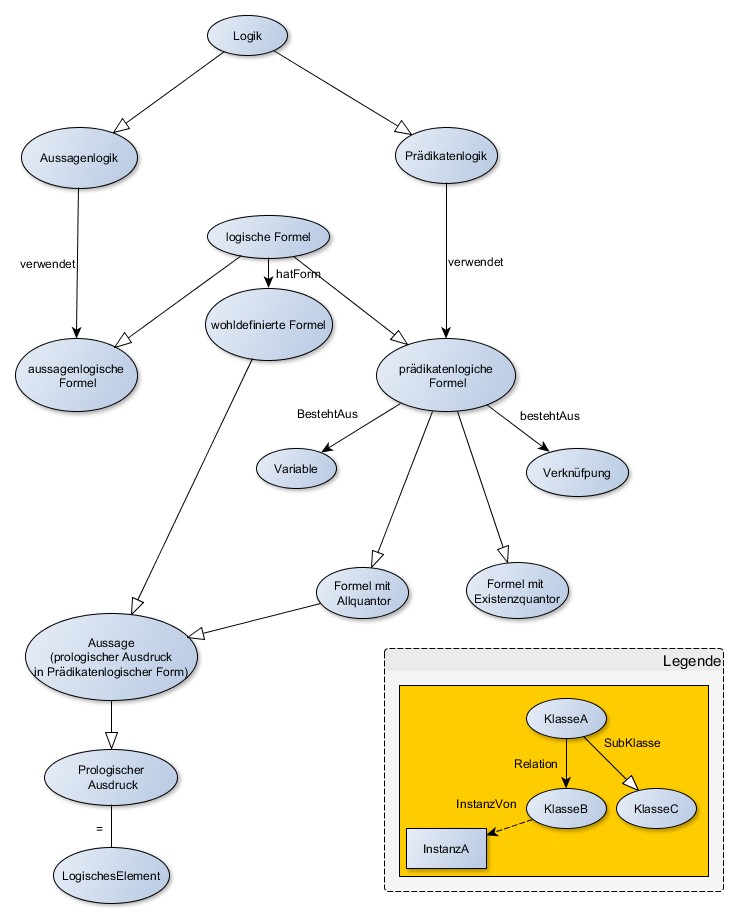
\includegraphics{bilder/formel_baum.png}}}
\caption{Vereinfachte Darstellung von Logik, rein mittels Klassen.\label{fig:prolog_logik_baum}\protect\footnotemark}
\end{figure}
\footnotetext{Eigene Darstellung mittels yEd.}

\newpage

Um auch Relationen abbilden zu können, wurde die Modellierung schliesslich mit Individuen erweitert. Dies erlaubte die Definition von Relationen zwischen diesen, was sich als Schritt in die richtige Richtung erweisen sollte.

\begin{figure}[H]
\centering \rotatebox{0}{\scalebox{0.3}[0.3]{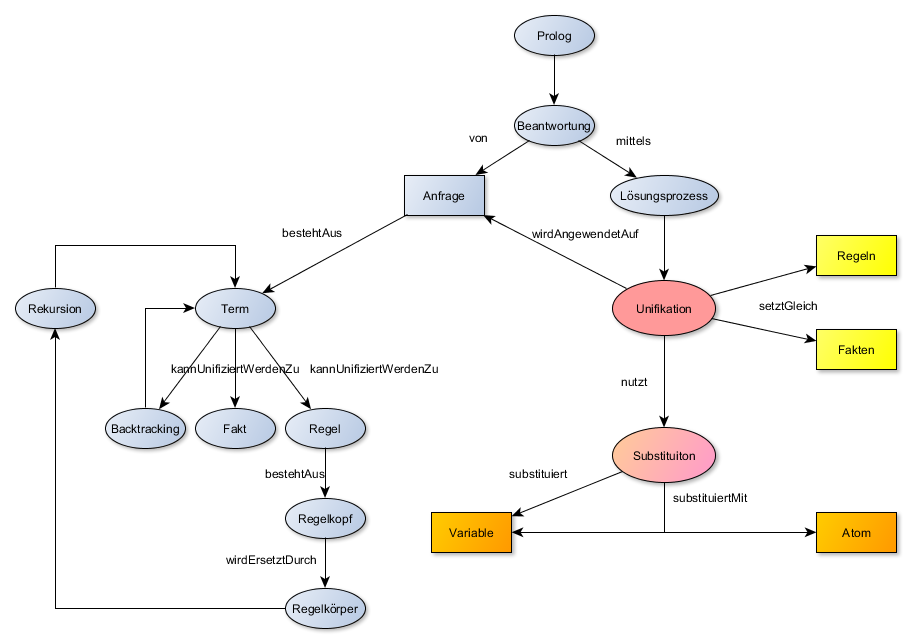
\includegraphics{bilder/loesungsprozess_baum.png}}}
\caption{Vereinfachte Darstellung eines Teils des Lösungsprozesses von Prolog, mittels Klassen, Individuen und Relationen.\label{fig:prolog_loesungsprozess}\protect\footnotemark}
\end{figure}
\footnotetext{Eigene Darstellung mittels yEd.}

Es wurde dann jeweils versucht konkrete Fragen aufgrund der erstellten Ontologie zu beantworten, wodurch Unvollständigkeiten in der Modellierung  sichtbar wurden. Diese zeigten sich zum Beispiel in Form von sehr umständlichen Abfragen um einfache Fakten zu erhalten. Details zu den gemachten Abfragen finden sich im Anhang~\ref{sec:anhang:sparql_beispiele}.

\begin{figure}[H]
\centering \rotatebox{0}{\scalebox{0.6}[0.6]{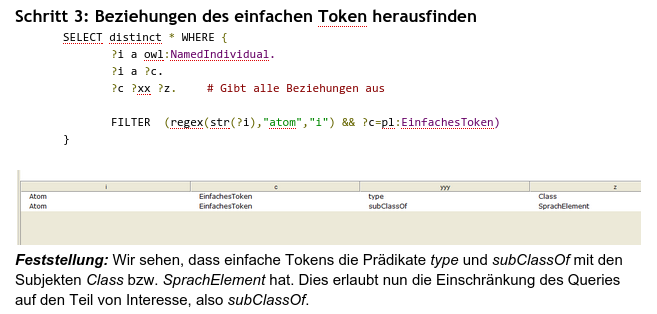
\includegraphics{bilder/sparql_beispiel.png}}}
\caption{Beispiel einer Abfrage der Ontologie mittels SPARQL.\label{fig:sparql_beispiel}\protect\footnotemark}
\end{figure}
\footnotetext{Eigene Darstellung mittels Stanford Protégé und Google Docs.}

Bei den genannten Mängeln handelte es sich nicht um Fehler. Grundsätzlich war es schwierig abzugrenzen bei welchem Detaillierungsgrad die Modellierung aufhören soll.So wurde schliesslich klar, dass bei einer zu feinen Granularität einer Modellierung, diese ins Uferlose gehen kann. Doch dies war nicht das Ziel, das Ziel war ein System zu schaffen, welches die Mächtigkeit dieser Art der Wissensmodellierung aufzeigt und damit Erfahrungen zu gewinnen. Daraufhin empfahl der Betreuer der Arbeit, Herr Dr.\ Eckerle, Literatur über Prolog als Grundlage bzw.\ Rahmen zu verwenden. Hierbei wurde auf das Buch \textit{Künstliche Intelligenz} von \textit{U. Lämmel} und \textit{J. Cleeve} zurückgegriffen~\cite{laemmel}. Herr Dr.\ Eckerle empfahl eine Beschränkung auf die Programmiersprache und deren Kernkonzepte, so wie sie auch im Buch beschrieben werden. Daraus resultierte eine verbesserte Modellierung der Ontologie von Prolog, mit Klassen, Relationen und Individuen.

\begin{figure}[H]
\centering \rotatebox{0}{\scalebox{0.15}[0.15]{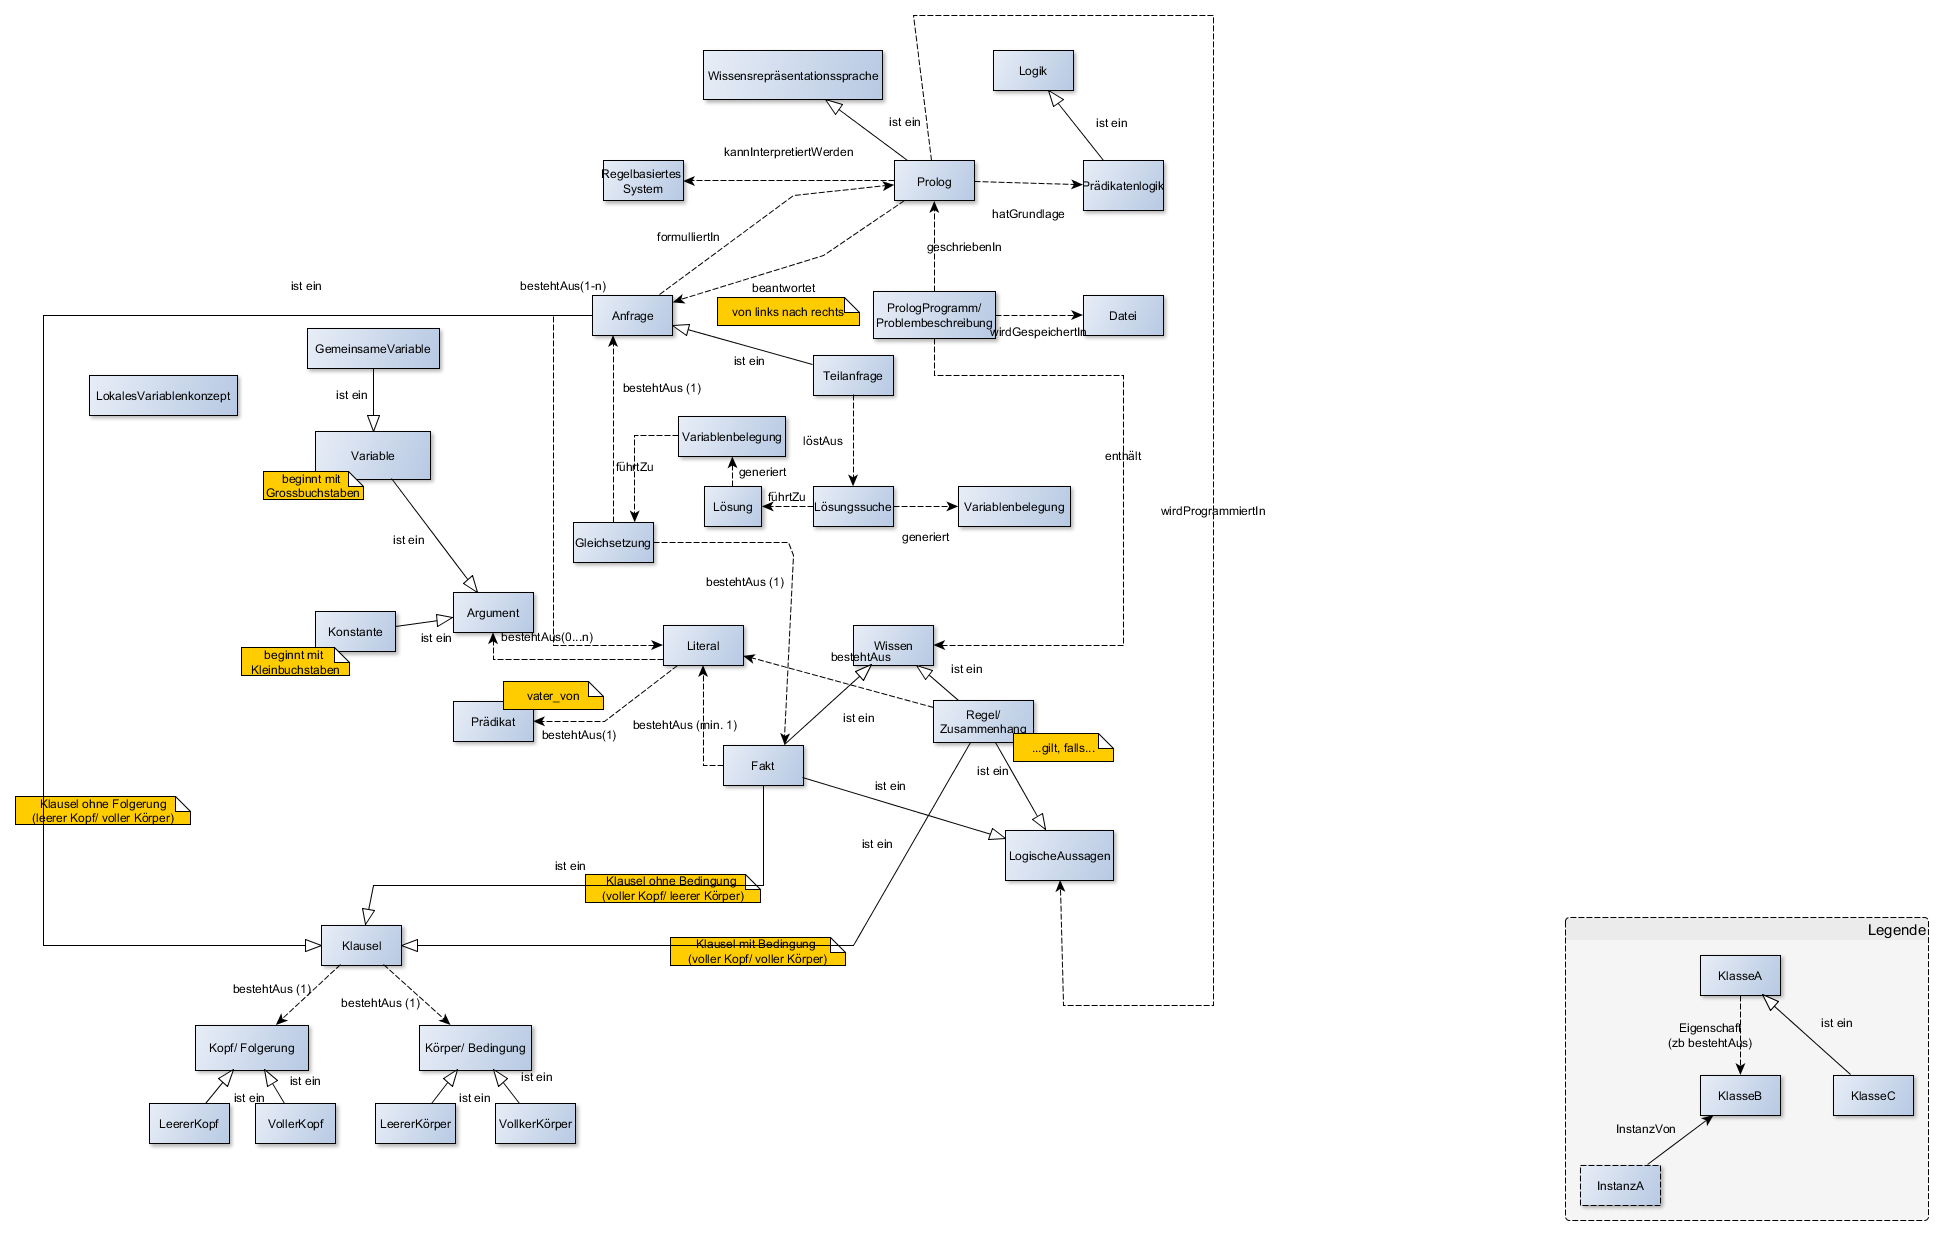
\includegraphics{bilder/prolog_baum.png}}}
\caption{Darstellung der Ontologie von Prolog, mit Klassen und Relationen (Individuen wurden der Übersicht halber bewusst weggelassen).\label{fig:prolog_baum}\protect\footnotemark}
\end{figure}
\footnotetext{Eigene Darstellung mittels yEd.}

Dies erlaubte jedoch nach wie vor keinen zusätzlichen Gewinn von Mehrwert in Form von Inferenz. Nach diversen Gesprächen mit Herrn Dr.\ Eckerle, stellte sich heraus, dass der Ontologie Regeln fehlen. Es wurde dann versucht mithilfe von Prolog das Konzept von Prolog abzubilden. Die Idee dahinter war, von der objektorientierten Denkweise loszukommen. Für die Autoren war es einfach nachzuvollziehen, dass und wie in Prolog Regeln verwendet werden. In Prolog wurde auch schnell deutlich, dass eine Abfrage auf Fakten (ohne Regeln) keinen Mehrwert bringt.

Nach diversen, erfolglosen Versuchen Regeln zu finden, wurde dies zuerst anhand einfacherer Modelle versucht. Zum Beispiel anhand eines Familienstammbaums. Mit diesem klassischen Beispiel wurde der Mehrwert der Wissensmodellierung mittels Ontologien sogleich erkannt.

\begin{figure}[H]
\centering \rotatebox{0}{\scalebox{0.15}[0.15]{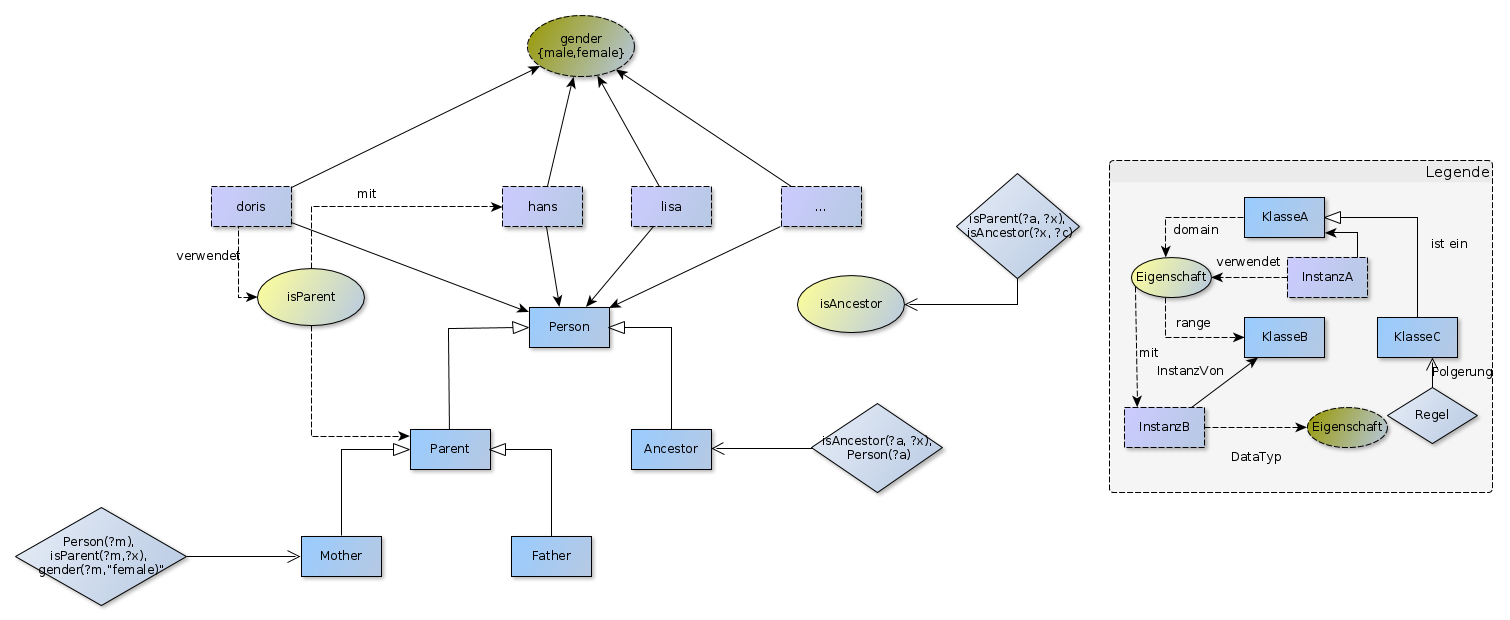
\includegraphics{bilder/familien_netz.png}}}
\caption{Ontologie eines Familienstammbaumes, mit Klassen, Individuen, Relationen und Regeln.\label{fig:familien_netz}\protect\footnotemark}
\end{figure}
\footnotetext{Eigene Darstellung mittels yEd.}

Es gelang nach dieser Erfahrung weiterhin nicht, Regeln für die eigentliche Wissensdomäne zu finden. Die Erkenntnis aus diesem Prozess war, dass die Abbildung von Prolog in einer Ontologie zwar möglich ist, jedoch eher in lexikalischer Form, was den Vorteil der Inferenz zu Nichte macht.

So kann beispielsweise gesagt werden, dass Prolog Unifikation auf Anfragen anwendet und dabei Regeln mit Fakten gleichsetzt. Dabei wird Substitution genutzt, welche Variablen mit Variablen und/oder Atomen substituiert. Dies wurde aber Grösstenteils in Form von Fakten abgebildet. Einige wenige Regeln konnten erzeugt werden.

Das damit abgebildete Wissen könnte aber auf eine einfachere und intuitivere Art mittels Fakten abgebildet werden. Somit ist der Mehrwert der Regel nichtig.

Nach eingehender Analyse kamen die Autoren zum Schluss, dass sich die gewählte Domäne nicht eignet, um die Mächtigkeit einer Ontologie und dem damit verbundenen Reasoning abzubilden. Für die Wissensmodellierung bzw. Expertensysteme eignen sich also eher Wissensdomänen, welche Probleme mit konkreten Objekten abbilden. Im Gegensatz dazu befindet sich die ursprünglich gewählte Domäne auf einer zu hohen Abstraktionsebene. Daher ist dort der konkrete Nutzen, in Form von Inferenz, nicht direkt sichtbar.

Wie der Name Expertensystem schon andeutet, werden diese in Fällen verwendet, bei denen ein Fachexperte notwendig ist. Dieser kann mit seinem Fachwissen Schlüsse ziehen und so zusätzliches Wissen generieren.

Daher wurde eine andere Wissensdomäne --- die Planung von Reisen --- gewählt. Dies geht bereits eher in die Richtung von Expertensystemen, wofür semantische Netze am ehesten geeignet scheinen.

Dieser Entscheidung gingen diverse Diskussionen und Versuche zur Wahl einer geeigneten Domäne voraus. So wurde zum Beispiel auch die Planung von Hochzeiten und medizinische sowie pharmazeutische Themengebiete in Betracht gezogen. Von diesen wurde jedoch abgesehen, da die Autoren in den Gebieten über zu wenig Fachwissen verfügen.

\begin{figure}[H]
\centering \rotatebox{0}{\scalebox{0.2}[0.2]{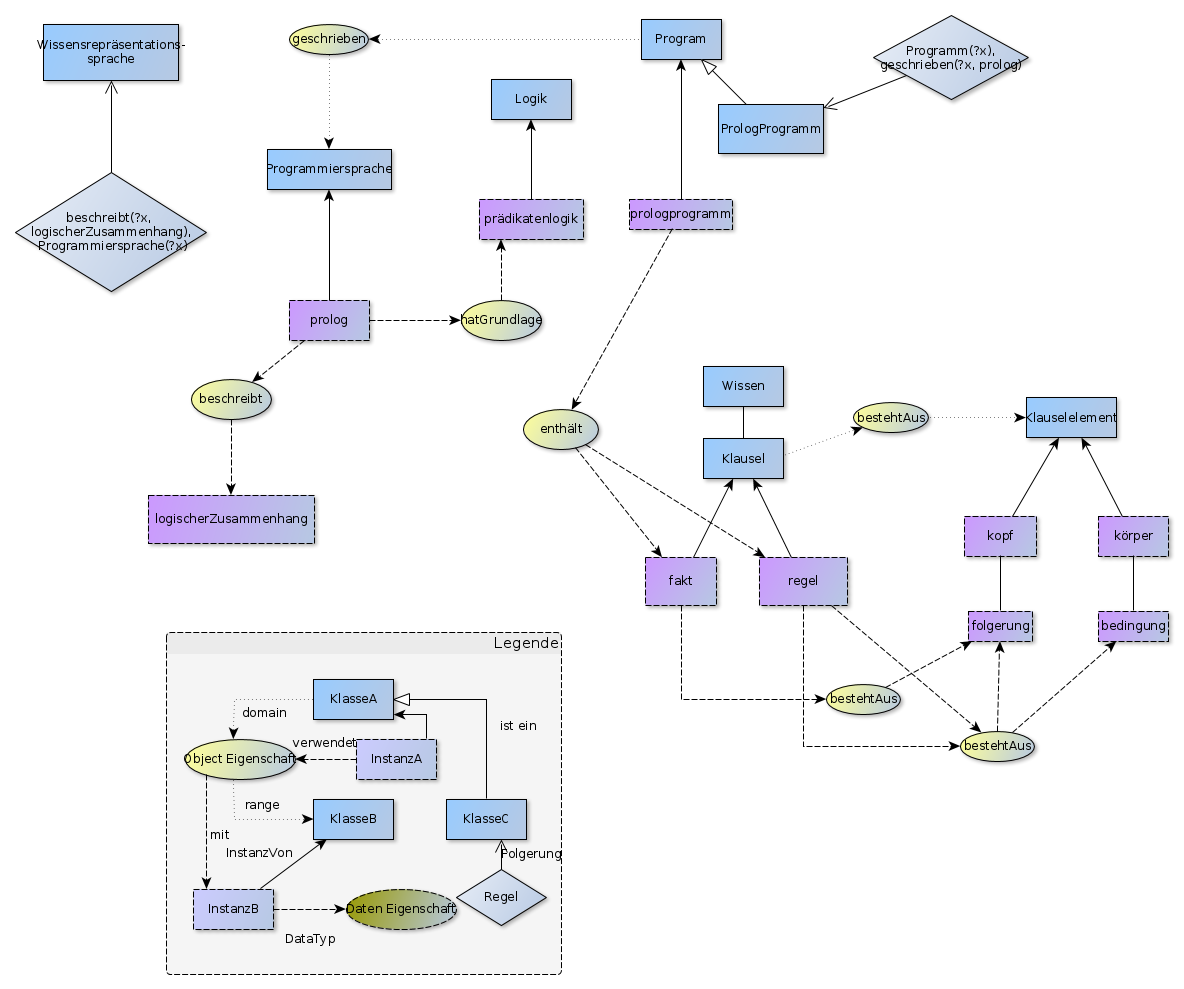
\includegraphics{bilder/prolog_netz.png}}}
\caption{Darstellung eines semantischen Netzes zur Abbildung von Prolog, mit Klassen, Individuen, Relationen und Regeln.\label{fig:prolog_netz}\protect\footnotemark}
\end{figure}
\footnotetext{Eigene Darstellung mittels yEd.}

\subsubsection{Modellierung der tatsächlichen Ontologie}
\label{sub:modellierung_der_ontologie_tatsaechliche}

Nach dieser Entscheidung wurde mit der Modellierung noch einmal beim Punkt null begonnen. Es konnte aber glücklicherweise auf den Erkenntnissen und Erfahrungen der vorigen Versuche aufgebaut werden.

Die Autoren entschieden sich anhand des gewonnen Wissens die Modellierung mittels konkreten Bespielen zu erarbeiten. Basierend auf diesen wurde die Ontologie erzeugt und stetig erweitert. Zur Veranschaulichung ein konkretes Beispiel:

\begin{lstlisting}[caption={Konkretes Beispiel einer Reiseplanung.},captionpos=b]
    Familie Muster plant einen eintägige Ausflug.
    Die Kinder sind in einem Alter in dem Sie immer beschäftigt sein müssen.
\end{lstlisting}

Im nachfolgenden Abschnitt findet sich eine Übersicht der Herleitung des Beispiels. Die Gedankengänge dahinter sind im Tutorial aufgeführt.

\newpage

Dies ergab eine noch sehr simple Ontologie, welche mit diesem semantischen Netz abgebildet werden kann:

\begin{figure}[H]
\centering \rotatebox{0}{\scalebox{0.5}[0.5]{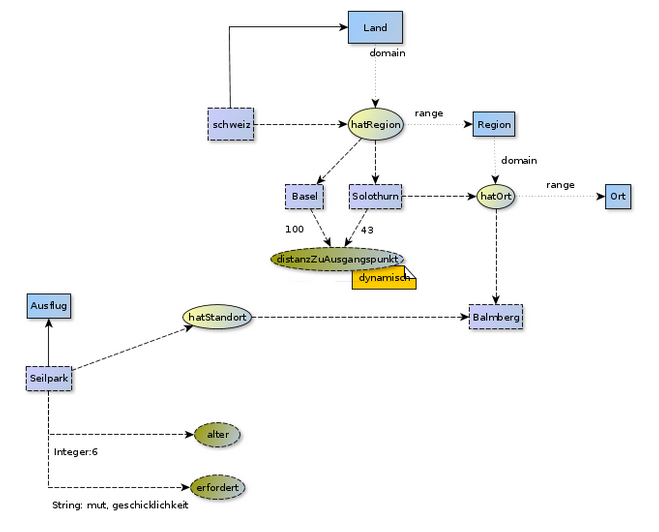
\includegraphics{bilder/famMuster.png}}}
\caption{Semantisches Netz für den Tagesausflug von Familie Muster.\label{fig:famMuster}\protect\footnotemark}
\end{figure}
\footnotetext{Eigene Darstellung mittels yEd.}

Mit der neu gewählten Wissensdomäne wurde auch der Sinn hinter der Verwendung von Regeln deutlich:
\begin{figure}[H]
    \centering \rotatebox{0}{\scalebox{0.5}[0.5]{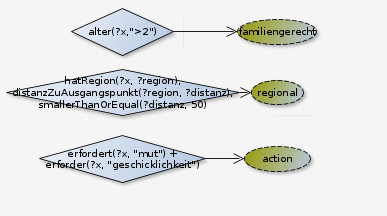
\includegraphics{bilder/famMusterRegeln.png}}}
    \caption{Regeln zum semantischen Netz für den Tagesausflug von Familie Muster.\label{fig:famMusterRegeln}\protect\footnotemark}
\end{figure}
\footnotetext{Eigene Darstellung mittels yEd.}

Aus der Modellierung konnten die folgenden Kriterien für die Abfrage abgeleitet werden:

\begin{itemize}
		\item familiengerecht
		\item action
		\item regional
\end{itemize}

Diese sind zugleich die Schlüsse der Regeln. Mit der richtigen SPARQL-Abfrage wird der Familie Muster schliesslich der Seilpark in Balmberg vorgeschlagen.

\begin{lstlisting}[caption={SPARQL-Abfrage um familiengerechte, regionale und actionreiche Ausflüge zu finden.},captionpos=b,language=SQL]
    SELECT
        *
    WHERE {
        ?object :familiengerecht true;
            :regional true;
            :action true.
        }
\end{lstlisting}


\begin{figure}[H]
\centering \rotatebox{0}{\scalebox{0.5}[0.5]{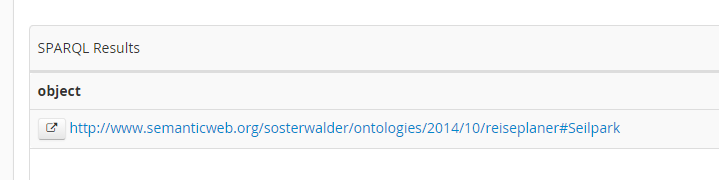
\includegraphics{bilder/famMusterOutput.png}}}
\caption{Ergebnis der Suche von Familie Muster.\label{fig:famMusterOutput}\protect\footnotemark}
\end{figure}
\footnotetext{Eigene Darstellung mittels yEd.}

In diesem ersten, bewusst sehr einfach gehaltenen Anwendungsfall, wird die Herangehensweise der Autoren sichtbar. Im Laufe von weiteren Beispielen wurde die Ontologie erweitert. So haben die Autoren zum Beispiel erst zu einem späteren Zeitpunkt eine Zeiteinheit eingeführt oder gemerkt, dass die Eigenschaft familiengerecht zu oberflächlich und pauschal betrachtet wurde. Diese wurde dahingehend geändert, dass die Eigenschaft Untereigenschaften beinhaltet, welche unterscheiden in welchem Alter die Kinder sind. Die gesamte Ontologie wird im~\autoref{sec:loesung_modellierung} genauer erläutert.

\subsection{Erstellung der Dokumentation zur Wissensmodellierung}
\label{subsec:dokumentation_wissensmodellierung}
Parallel zur Modellierung der Ontologie entstand ein Tutorial, welches aufzeigt, wie ein Knowledge Engineer vorgeht um eine Problemdomäne systematisch zu modellieren und formalisieren. Wie bereits zuvor erwähnt, wurde als Problemdomäne die Planung von Reisen gewählt. Das Tutorial findet sich im Anhang unter~\ref{sec:anhang:tutorial_dokument}.

\subsubsection{Aufbau des Tutorials}
\label{subsec:dokumentation_wissensmodellierung_aufbau}
Im Gegensatz zu herkömmlichen Tutorials enthält das in dieser Arbeit erstellte einen grossen Theorieanteil. Aus diesem Grund wurde das Dokument in drei Aspekte aufgeteilt.

Da es sich hierbei um eine wissenschaftliche Arbeit handelt, haben die Autoren entschieden in einem ersten Teil theoretisches Hintergrundwissen zur Wissensmodellierung bereitzustellen. So wird zum Beispiel erläutert was Expertensysteme sind, wie diese grafisch dargestellt werden können und welche Schreibweisen respektive Sprachen verwendet werden um eine Ontologie abzubilden und darauf Abfragen zu stellen.

\noindent\rule[1ex]{\textwidth}{1pt}
\begin{wrapfigure}[4]{l}{0.1\textwidth}
    \vspace{-18pt}
    
\includegraphics[width=0.1\textwidth]{bilder/owl.png}
\end{wrapfigure}
Durch das Symbol der Eule wird die zweite Herangehensweise im Dokument eingeleitet. Im jeweils danebenstehenden Abschnitt sind praktische Hinweise zur aktuellen Thematik aufgeführt.\\
\noindent\rule[1ex]{\textwidth}{1pt}

\noindent\rule[1ex]{\textwidth}{1pt}
\begin{wrapfigure}[4]{l}{0.1\textwidth}
    \vspace{-18pt}
    
\includegraphics[width=0.1\textwidth]{bilder/elephant.png}
\end{wrapfigure}
Der letzte Teil des Dokumentes, welcher durch das Symbol des Elefanten gekennzeichnet ist, verkörpert ein Tutorial im klassischen Sinne. Einem pragmatisch veranlagten Leser ist es so möglich, durch Folgen des Symbols, innerhalb von kurzer Zeit ein simples Beispiel eines Expertensystemes aufzubauen.\\
\noindent\rule[1ex]{\textwidth}{1pt}

\subsection{Erstellung der abschliessenden Dokumentation}
\label{subsec:abschliessende_dokumentation}
Mit der Erstellung der abschliessenden Dokumentation ist das hier vorliegende Dokument gemeint. Dieses wurde während der ganzen Projektarbeit stetig erweitert, auch um die bereits fertiggestellten Arbeiten zu reflektieren. Als Grundlage für das Dokument diente das bereits erwähnte Dokument, in welchem die Autoren ihre Erkenntnisse fortlaufend festhielten.

\chapter{Lösung}
\label{chap:loesung}
% In diesem Kapitel beschreiben Sie Ihre Lösung des Problems. Geben Sie dem Leser genügend Einblick in die Lösung, so dass er Ihre Arbeit entsprechend würdigen kann. Verwenden Sie aber Anhänge für Dinge, die hier nicht unbedingt bis ins letzte Detail verstanden werden müssen.
Die Aufgabenstellung beschreibt das Ziel dieser Bachelor Thesis mit dem einfachen Satz ``Ziel dieser Arbeit ist die Entwicklung und Anwendung eines Systems zur Speicherung (von Daten) in einer semantischen Datenbank$\cdots$''.~\cite{Aufgabenstellung} Es sollen also Daten in einem Datenspeicher abgelegt werden. Der einzig unbekannte Faktor ist dabei, dass es sich bei der Datenbank um eine semantische Datenbank handeln soll. Bei genauerer Betrachtung wird interessierten Personen bewusst, das sich Einiges dahinter verbirgt.

Auf der einen Seite eine Ansammlung von neuen Technologien und Theorien. Auf der anderen Seite eine völlig unbekannte und vor allem ungewohnte Denkweise, welche erst erkannt und dann auch angewendet werden muss. Dies ist gerade für Personen aus der Informatik, speziell mit objektorientiertem Hintergrund eine Herausforderung. Die Erfahrungen und Schwierigkeiten dabei werden im~\autoref{sub:modellierung_der_ontologie} beschrieben.

Eine Anforderung, welche bei der Spezifikation der Meilensteine nicht erwähnt wurde, ist der Anspruch der Autoren innerhalb einer gewissen Wissensdomäne Fragen beantworten zu können. Dies impliziert bereits fundiertes Fachwissen der Thematik, da Fragen anhand der Semantik der Inhalte beantwortet werden sollen. 

Die Organisation sowie die Herangehensweise der Autoren wurden im \autoref{chap:administratives} und \autoref{chap:vorgehen} ausführlich beschrieben. In diesem Kapitel liegt der Fokus auf der tatsächlichen Lösung der Anforderungen.

\section{Von der Wissenserarbeitung zum Tutorial}
\label{sec:loesung_tutorial}
Um die oben erwähnten Technologien, Sprachen und Theorien zu erarbeiten und diese vor allem mit dem Leser zu teilen, wurde ein Tutorial erarbeitet. Dabei war es schwierig ein einfach nutzbares Tutorial zu erstellen, dem Leser dabei aber auch genügend Hintergrundwissen zu vermitteln. Der Leser soll wirklich verstehen können was hinter einer Wissensmodellierung respektive einem Expertensystem steckt. Daraus entstand ein Dokument, welches die Modellierung aus drei Perspektiven beleuchtet. Diese werden ausführlich im \autoref{subsec:dokumentation_wissensmodellierung_aufbau} beschrieben.

\section{Modellierung}
\label{sec:loesung_modellierung}

Semantische Datenbanken werden auf Basis von Ontologien gebildet. Eine Ontologie wird für eine Problemdomäne erstellt und bildet ihr Wissen ab. Die Problemdomäne dieser Arbeit ist das Reisen. Es wurde entschieden sich vorerst auf Ausflüge in der Schweiz zu begrenzen. Damit ist es möglich die Mächtigkeit eines Expertensystems aufzuzeigen. Die gesamte Modellierung wurde mithilfe von OWL formuliert. Bei OWL handelt es sich um eine Ontologieabbildungssprache. Benötigte Regeln werden in der Regelsprache SWRL formuliert. Details dazu können im~\hyperref[sec:anhang:tutorial_dokument]{Tutorial} unter Kapitel 9 nachgelesen werden.

Zur Veranschaulichung wurde jeder Teil der Ontologie und die dazugehörigen Regeln in einem semantischen Netz abgebildet. Sämtliche Grafiken finden sich als Anhang unter~\ref{sec:anhang:grafiken}.

%\begin{figure}[H]
%\centering \rotatebox{0}{\scalebox{0.3}[0.3]{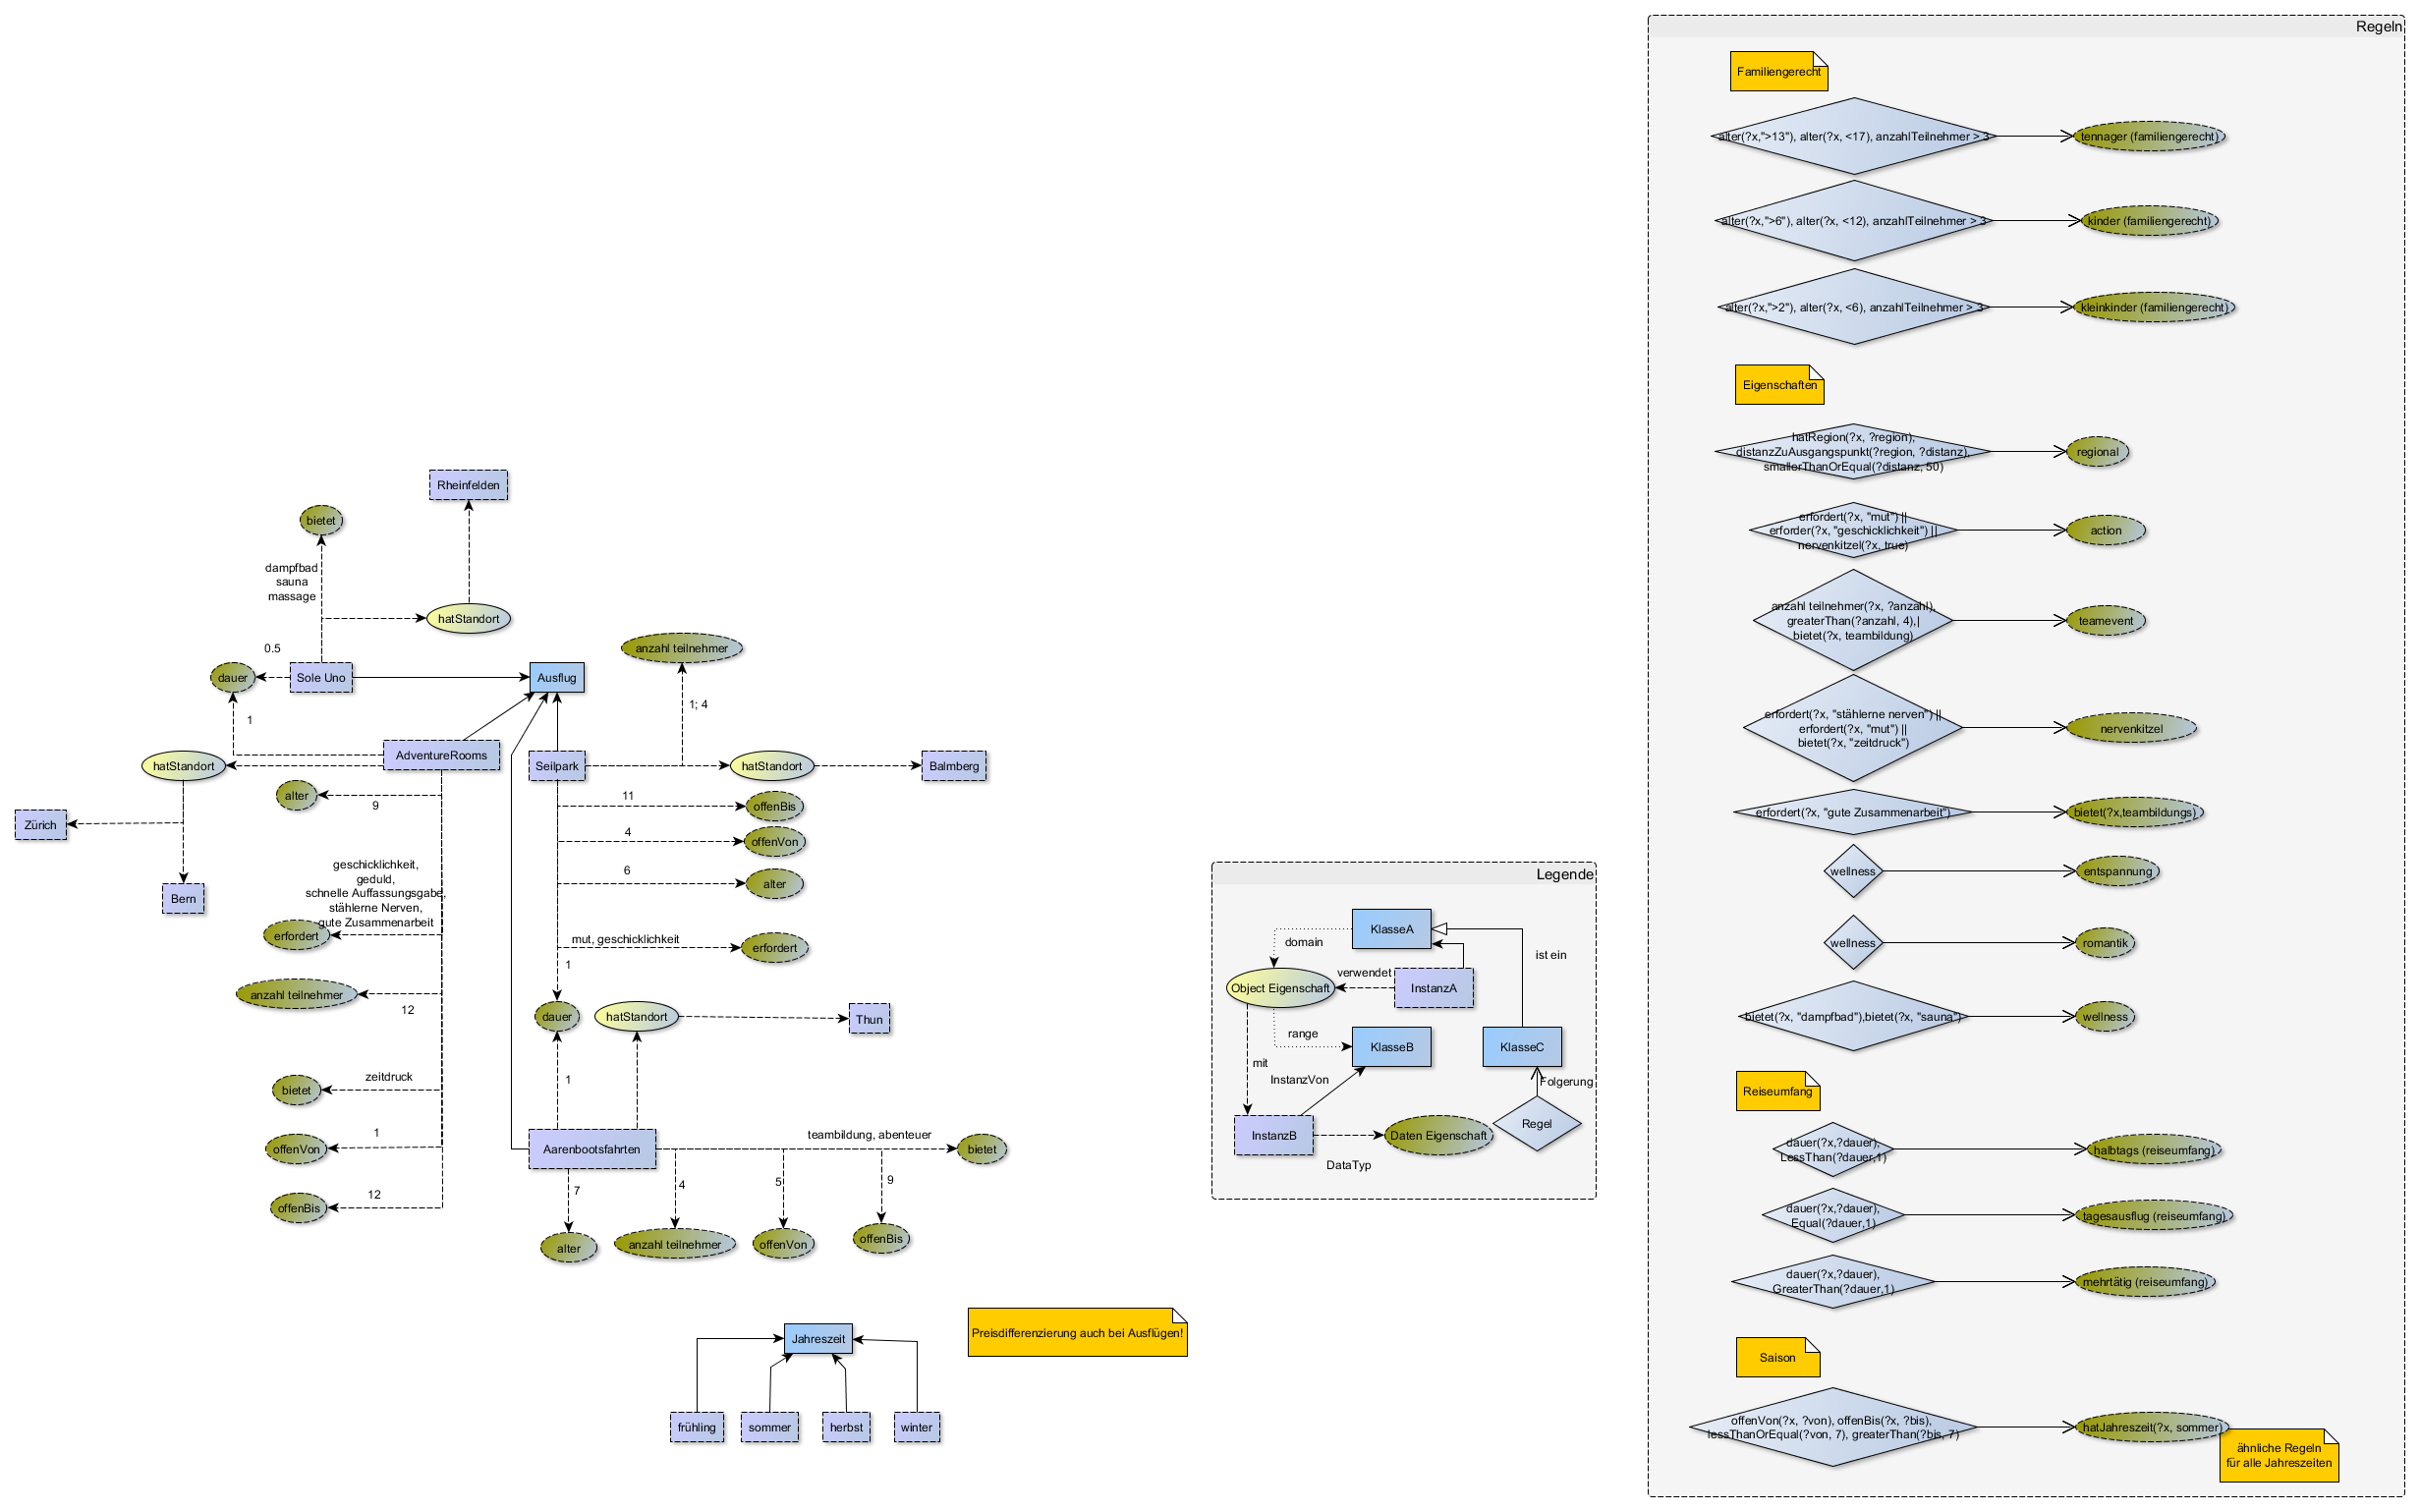
\includegraphics{bilder/semNetzLoesung.png}}}
%\caption{Ausschnitt des semantischen Netzes zur Abbildung der Ontologie.\label{fig:semNetzLoesung}\protect\footnotemark}
%\end{figure}
%\footnotetext{Eigene Darstellung mittels yEd.}


Durch die Beschränkung der Problemdomäne auf Tages- und Wochenendausflüge in der Schweiz, konnten zwei Hauptkomponenten (Ausflüge und Restaurants) extrahiert werden.

Sowohl ein Restaurant als auch ein Ausflug werden durch Eigenschaften von Bedingungen (Bedingungsproperty) beschrieben. Ein Restaurantbesitzer könnte also dem Betreiber des erstellten Reiseplaners die Qualitäten seines Restaurants angeben. Diese Eigenschaften gehen von der Beschreibung des Ambientes, über kulinarischen Spezialitäten zu den durchschnittlichen Preisen, welche das Restaurant hat. Der Ausflug ist durch andere Werte wie der Anzahl Teilnehmer, den Öffnungszeiten oder was ein Ausflug bietet oder erfordert beschrieben.
Mittels Regeln ist festgelegt welche Folgerungen aus diesen Eigenschaften abgeleitet werden können.

    \begin{figure}[H]%[htbp]
        \begin{minipage}[hbt]{0,49\textwidth}
            \centering
            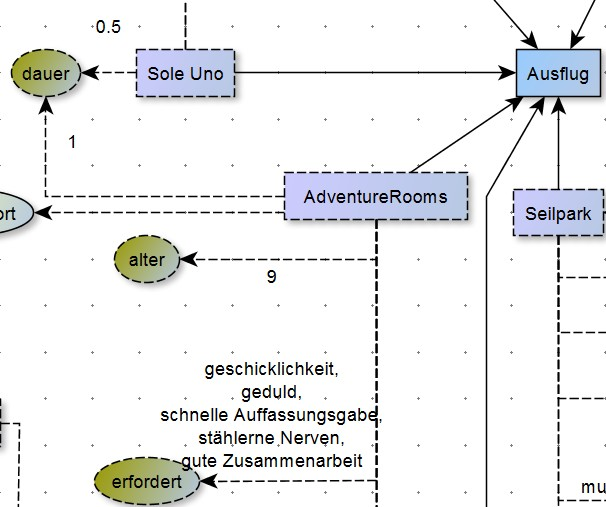
\includegraphics[scale=0.3]{bilder/charAusflug.jpg}
            \caption*{Eigenschaften eines Ausflugs.\label{fig:charAusflug}\protect\footnotemark}
        \end{minipage}
        \begin{minipage}[hbt]{0,49\textwidth}
            \centering
            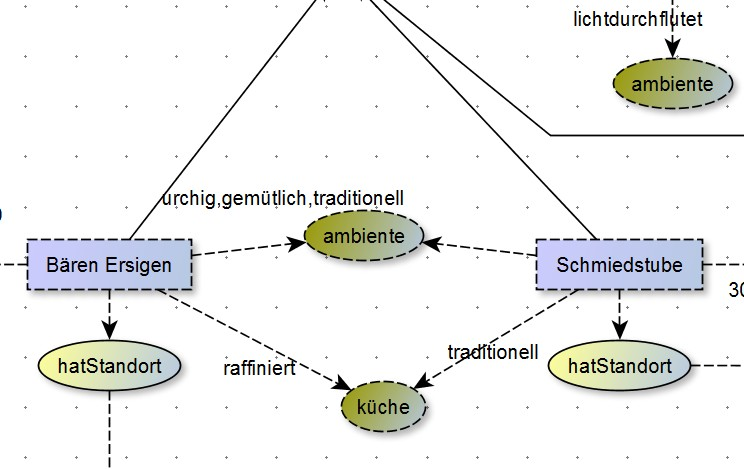
\includegraphics[scale=0.3]{bilder/charRestaurant.jpg}
            \caption*{Eigenschaften eines Restaurants.\label{fig:charRest}\protect\footnotemark[1]}
        \end{minipage}
    \end{figure}
\footnotetext{Eigene Darstellung mittels yEd.}

Um die verschiedenen Möglichkeiten beim Abbilden einer Ontologie aufzuzeigen, wurde für die Spezifikation der Hauptkomponenten jeweils eine andere Umsetzung gewählt. Die Klasse Restaurant hat verschiedene Unterklassen. Der Besucher hat also bei der Suche die Auswahl zwischen verschiedenen Typen von Restaurants zur Verfügung. Je nach gewähltem Typ müssen unterschiedliche Kriterien (Bedinungsproperties) erfüllt sein. So ist zum Beispiel festgelegt, dass eine raffinierte Küche mit frischen und saisonalen Speisen auf ein Gourmetrestaurant schliessen lässt.

Wenn also in diesem Fall der Benutzer auswählt, dass er ein Gourmetrestaurant sucht, würden nur jene Restaurants ermittelt, welche als Eigenschaften raffinierte Küche mit frischen und saisonalen Speisen aufweisen. Das Preissegment ist als Klasse mit Individuen definiert. Jedes Individuum stellt da bei ein Preissegment dar. Liegt der Durchschnittspreis eines Restaurants in einem bestimmten Rahmen so definieren Regeln in welchem Preissegment das Restaurant liegt.  Dies ist durch eine Eigenschaft des Objektes (ObjectProperty) festgelegt. Objekteigenschaften beschreiben die Beziehungen zwischen zwei Individuen.

Bei den Ausflügen werden dem Benutzer des Reiseplaners Schlussfolgerungen angeboten. Mittels der vorher erwähnten Regeln ist festgelegt welche Bedienungen zutreffen müssen um eine gewisse Eigenschaft zu erfüllen. So ist zum Beispiel festgelegt, dass ein Ausflug der Wellness bietet entspannend und romantisch ist.\\
Sowohl Folgerungen als auch Bedingungen werden in Form von so genannten DataProperties definiert. Diese legen eine Eigenschaft eines Individuums fest.

    \begin{figure}[H]%[htbp]
        \begin{minipage}[hbt]{0,49\textwidth}
            \centering
            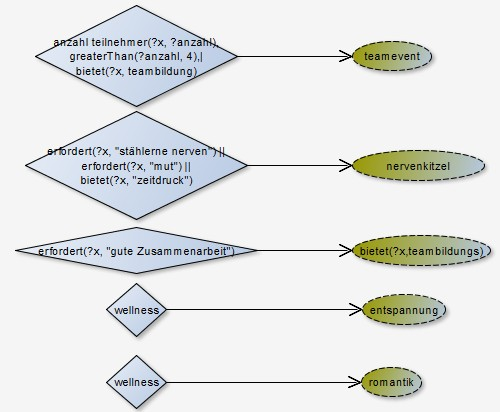
\includegraphics[scale=0.3]{bilder/AufbauAusflug.jpg}
            \caption*{Schlussfolgerungen Ausflug.\label{fig:AufbauAusflug}\protect\footnotemark[1]}
        \end{minipage}
        \begin{minipage}[hbt]{0,49\textwidth}
            \centering
            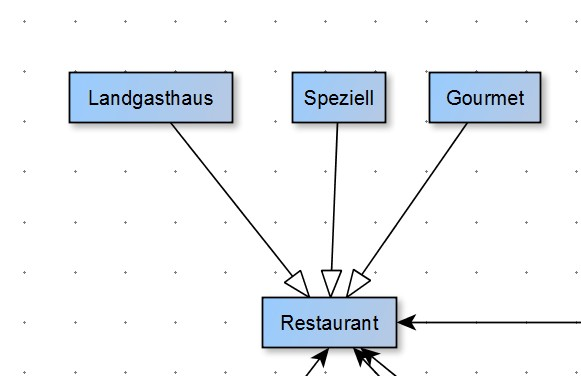
\includegraphics[scale=0.3]{bilder/AufbauRest.jpg}
            \caption*{Restaurant Typen.\label{fig:AufbauRest}\protect\footnotemark[1]}
        \end{minipage}
    \end{figure}
\footnotetext{Eigene Darstellung mittels yEd.}

In beiden Fällen ist zu beachten, dass der Benutzer sich entscheiden kann, ob er entweder eine von der Region oder von dem Ort abhängige Einschränkung für die Suche festlegen möchte. Die Beziehung zwischen den Region/Orten und den konkreten Ausflügen/Restaurants wird mit Hilfe von ObjectProperties erreicht. Es wird also zum Beispiel gesagt, dass ein Ausflug den Standort Bern hat. Als Erweiterung kann der Benutzer festlegen, dass er ein Restaurant sucht, welches sich im gleichen Ort respektive in der gleichen Region befindet wie der Ausflug.\\

Eine Besonderheit von Ausflügen ist, dass sie nicht das ganze Jahr über machbar sind. Durch eine Eigenschaft eines Ausfluges (DataProperty) kann der Betreiber festlegen in welchem Zeitraum ein Ausflug machbar ist (offen von bis).Dank geeigneter Regeln wird abgeleitet in welcher Saison ein Ausflugsziel für Besucher offen ist. Dazu wurde eine Klasse Jahreszeiten mit entsprechenden Individuen eingeführt.\\
    \begin{figure}[H]%[htbp]
        \begin{minipage}[hbt]{0,49\textwidth}
            \centering
            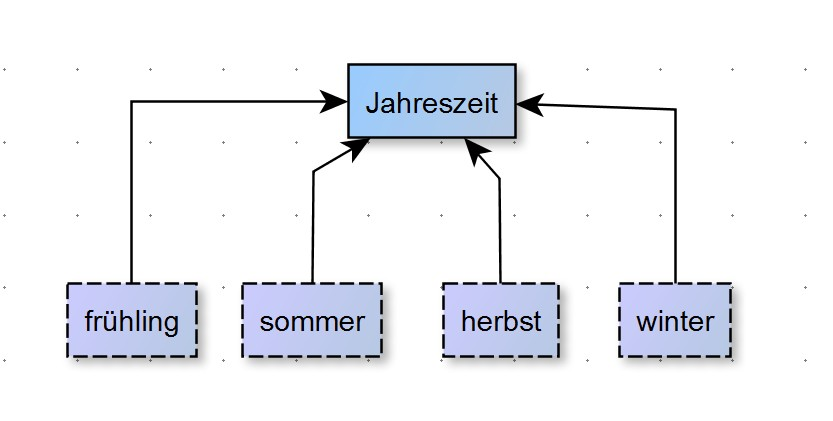
\includegraphics[scale=0.3]{bilder/SaisonKlasse.jpg}
            \caption*{Abbildung der Jahreszeiten.\label{fig:SaisonKlasse}\protect\footnotemark}
        \end{minipage}
        \begin{minipage}[hbt]{0,49\textwidth}
            \centering
            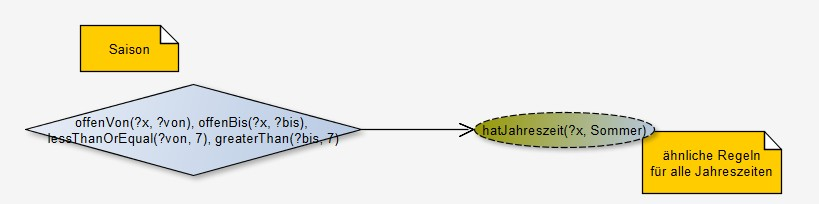
\includegraphics[scale=0.3]{bilder/SaisonRegeln.jpg}
            \caption*{Regel zur Bestimmung der Jahreszeiten.\label{fig:SaisonRegeln}\protect\footnotemark[2]}
        \end{minipage}
    \end{figure}


Ein ähnliches Prinzip wurde angewendet um die Ruhetage eines Ausflug beziehungsweise eines Restaurants abzubilden. Für jede Reisedestination kann der Organisator angegeben, welche Ruhetage sie hat. Regeln legen fest, dass die Reise an einem Tag machbar ist, wenn der Tag kein Ruhetag ist. Dies ist eher umständlich und nicht sehr intuitiv umgesetzt. Vor allem da bei einem Ausflug der täglich ausgeführt werden kann der Ruhetag 8 angegeben werden muss (eine Zahl die nicht zwischen 1-7 also Montag bis Sonntag liegt). Hiermit wollten die Autoren die Einschränkung von Wissensmodellierungen mittels Ontologien aufzeigen, dass in Regeln keine Negationen möglich sind. Auf der Anderen Seite zeigt diese Methode den Vorteil solcher Modellierungen auf. Sie können erweitert werden, ohne das der Programmcode angepasst werden muss. Da es ja möglich ist, die Daten mit eigener Logik zu versehen. 

Eines der grösseren Probleme bei der Modellierung war die zeitliche Beschränkung. Bekanntlich kann dem Lösen von Planungsproblemen, welche NP-vollständig sind, eine ganze Bachelor Thesis gewidmet werden. Erschwerend kommt dazu, dass es bei der Wissensabbildung mittels OWL nur in sehr begrenztem Rahmen möglich ist zu rechnen. Da dies kein wichtiger Teil der Arbeit ist, haben die Autoren entschieden, dass es keinen Sinn macht diese Problematik in Form von Programmlogik zu lösen. Aus diesem Grund fällt die Zeitplanung relativ simpel aus. Es kann festgelegt werden wie viel Zeit ein Ausflug in Anspruch nimmt. In der Verwendung kann der Benutzer des Reiseplaners angeben wie viel Zeit er für einen Ausflug zur Verfügung hat. Zur Auswahl stehen die Kriterien halbtags, ganztags und mehrtägig, wobei die mehrtägigen Ausflüge nicht eingearbeitet wurden. In dieser Version des Reiseplaners werden in der Anfrage immer nur jene Ausflüge ausgegeben, welche der festgelegten Zeiteinheit entsprechen. Um die Dauer eines Ausfluges flexibler zu gestalten haben die Autoren entschieden, dass mehrere Male das Dauer-attribut gesetzt werden kann. Mit dieser Erweiterung kann ein Ausflug sowohl als halb als auch als ganztägiger deklariert werden.

    \begin{figure}[H]%[htbp]
        \begin{minipage}[hbt]{0,49\textwidth}
            \centering
            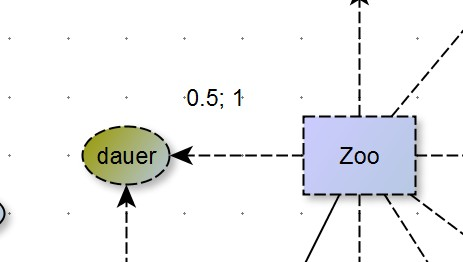
\includegraphics[scale=0.3]{bilder/dauer.jpg}
            \caption*{Dauer eines Ausflugs festlegen.\label{fig:dauer}\protect\footnotemark[2]}
        \end{minipage}
        \begin{minipage}[hbt]{0,49\textwidth}
            \centering
            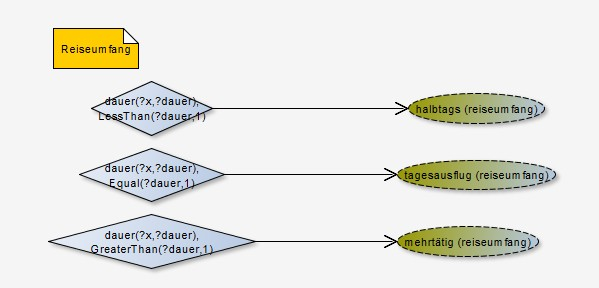
\includegraphics[scale=0.3]{bilder/reiseUmfang.jpg}
            \caption*{Regel zur Bestimmung des Reiseumfangs.\label{fig:reiseumfang}\protect\footnotemark[2]}
        \end{minipage}
    \end{figure}
\footnotetext{Eigene Darstellung mittels yEd.}

\subsection{Mängel in Stardog}
\label{subsec:loesung_modellierung_maengel_stardog}
Im Laufe der Modellierung sind die Autoren auf ein für sie unerklärliches Phänomen gestossen. So war es dem Reasoner in Stardog nicht möglich von einem DataProperty auf dasselbe DataProperty zu schliessen. Konkret wollten die Autoren aussagen, dass ein Ausflug, der eine Sauna bietet auch Wellness bietet. Diese Regel kann aber von Stardog nicht ausgewertet werden. In Protégé wird die Schlussfolgerung aber richtig angezeigt. Nach längeren Recherchen befanden die Autoren, dass es sich bei dieser Einschränkung wohl um einen technischen Fehler von Stardog handeln muss. Dagegen sprach allerdings, dass beide Werkzeuge den gleichen Reasoner (Pellet) verwenden. Nach dem Melden des Fehlers (Bugreporting) in der Diskussionsgruppe von Stardog, erhielten die Autoren die Information, dass es sich tatsächlich um einen Fehler des Systems handelt. Anscheinend wurde ein zu strenges Ausschlussverfahren in der Programmlogik angewendet um zirkuläre Referenzen zu vermeiden. Dies soll aber im nächsten Release korrigiert werden. \\
Also Workround wurde die Modellierung von den Autoren so abgeändert, dass Wellness ein DataProperty vom Typ Boolean ist. Da es sich so nicht mehr um dasselbe DataProperty handelt, funktioniert die angepasste Regel.

\subsection{Ergebnis}
\label{subsec:loesung_modellierung_ergebnis}
Ein Teil des Ergebnisses der Modellierung sind die oben erwähnten semantischen Netze. Diese wurden in drei Grafiken aufgeteilt. Auf der ersten Grafik wird die gesamte Region/Ort-Thematik abgebildet. Auf zwei weiteren Grafiken wurden jeweils die Details zu den Restaurants respektive Ausflügen dargestellt.

Der zweite Teil ist ein von Protégé generiertes RDF/XML-Dokument. Darin ist die semantische Datenbank im OWL-Format abgelegt. Es handelt sich dabei um die konkreten Daten.

\section{Erstellung von Abfragen}
\label{sec:loesung_sparql}
Sowohl während des Abbildens der Problemdomäne, als auch für die endgültige Suche, mussten immer wieder Abfragen erstellt werden. Abfragen müssen in einer semantischen Datenbank mittels SPARQL gestellt werden. Dabei handelt es sich um eine Abfragesprache für Ontologien. Details dazu finden sich im~\hyperref[sec:anhang:tutorial_dokument]{Tutorial} unter Kapitel 10. Die Abfragen sind direkt in der erstellten Benutzeroberfläche integriert. So konnte verhindert werden, dass der Benutzer gezwungen ist, sich die Sprache anzueignen.

\section{Benutzeroberfläche}
\label{sec:loesung_gui}
Eine weitere Anforderung an die Lösung lautet ``\ldots Besondere Bedeutung kommt dabei der Schnittstelle zwischen Mensch und System zu \ldots''.~\cite{Aufgabenstellung}

Da klar wurde, dass es in keiner Weise benutzerfreundlich ist, Abfragen mittels SPARQL zu schreiben, wurde eine Webapplikation zur Reiseplanung entwickelt. Dabei wird der Benutzer des Reiseplaners mit Hilfe eines Assistenten durch die Auswahl geführt. Neben der Vermeidung von SPARQL während der Benutzung, ist so sichergestellt, dass der Benutzer nur Abfragen stellen kann, welche wenigstens in der Theorie Sinn ergeben.

In einem ersten Schritt kann der Benutzer entscheiden ob er nur ein Ausflug planen will oder auch nach einem Restaurant sucht. Im zweiten Schritt werden sämtliche gefolgerte Eigenschaften und Beziehungen zu den gewählten Komponenten angeboten. Zum Schluss erhält der Benutzer eine Liste sämtlicher Ergebnisse. Dabei wird aus allen gewählten Eigenschaften dynamisch eine SPARQL-Abfrage generiert. In der Ausgabe sind der Name des Ausflugs, sein Standort und, wenn vorhanden, die URL zu seiner Homepage aufgelistet. Je nach Kriterien ist es natürlich möglich, dass keine Reise gefunden wird. Dies ist der Fall, wenn keine der erfassten Reisen auf die gewählten Kriterien zutrifft. Da nur sehr exemplarisch Reisen erfasst wurden, ist das Risiko für eine leere Antwort relativ hoch.
\begin{figure}[H]
\centering \rotatebox{0}{\scalebox{0.3}[0.3]{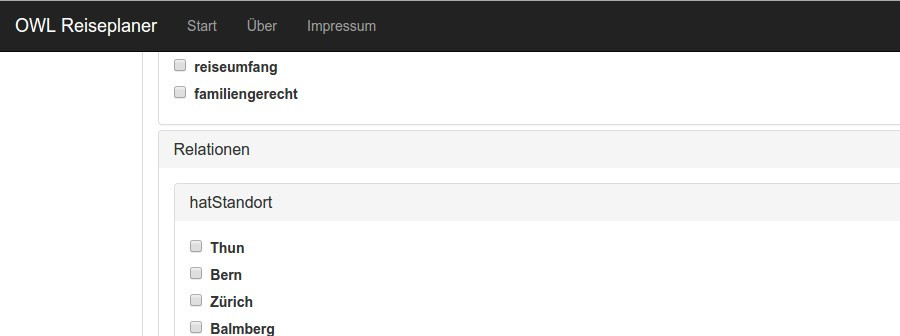
\includegraphics{bilder/reiseplaner_gui.jpg}}}
\caption{Ausschnitt der Benutzeroberfläche. Schritt Zwei des Assistenten.\label{fig:gui}\protect\footnotemark}
\end{figure}
\footnotetext{http://elephantsearch.bfh.ch:5820/}

\chapter{Komponenten}
\label{chap:komponenten}
Ein Expertensystem besteht aus drei Komponenten, wie im~\hyperref[sec:anhang:tutorial_dokument]{Tutorial} unter Kapitel 2 beschrieben.\\
Die Komponenten sind:
\begin{itemize}
    \item Wissensdatenbank: Enthält die Fakten des Problembereiches in formaler Sprache
    \item Inferenz-Maschine: Verarbeitungsmechanismus zum automatischen Ziehen von Schlüssen
    \item Benutzerschnittstelle
\end{itemize}
Wie in~\autoref{ssubsec:vorgehen:grundlagen:technisch} erwähnt, ist die Verwendung von Werkzeugen zur Modellierung einer Ontologie sinnvoll.\\
Dabei gibt es Überschneidungen: \textbf{Komponenten können auch Werkzeuge sein.}

Das folgende Kapitel beschreibt die während dieser Arbeit verwendeten Komponenten und Werkzeuge.

Die Wissensmodellierung sollte ursprünglich mit Hilfe von Apache Stanbol umgesetzt werden, wie unter~\autoref{ssubsec:vorgehen:grundlagen:technisch} erwähnt. Während der Arbeit wurde erkannt, dass diese Technologie für die vorgesehene Aufgabe nur bedingt sinnvoll ist. In Apache Stanbol ist es zwar möglich die modellierte Wissensdomäne zu importieren. Das importierte Modell wird als Ontologie in Form von Tripeln gespeichert. Die Objekte, ihre Eigenschaften sowie Relationen lassen sich jedoch nicht verwalten.

Für Anfragen an die Wissensdatenbank ist eine entsprechende Schnittstelle notwendig. Von Apache Stanbol wird diese Schnittstelle in Form eines SPARQL-Endpoints zur Verfügung gestellt. Der SPARQL-Endpoint nutzt jedoch die ContentHub-Komponente von Apache Stanbol als Datenbasis. Diese stellt nur Wissen zur Verfügung, welches aus angereicherten Inhalten abgeleitet ist. Mittels Ontologien und Regeln werden diese Inhalte angereichert.

Eine aufwändige Recherche ergab: Anderen Datenquellen können für den SPARQL-Endpoint genutzt werden. Dies bedeutet jedoch einen erheblichen Mehraufwand in Form einer eigenen Implementation.

Damit war Apache Stanbol nicht das geeignete Werkzeug für diese Arbeit. Bei weiteren Recherchen wurden weitere Werkzeuge gefunden, welche als Ersatz für Apache Stanbol genutzt werden konnten: \textit{Protégé} der Universität Stanford sowie \textit{Stardog} der Firma Clark \& Parsia.

\section{Stanford Protégé}
\label{sec:komponenten_protege}
Protégé ist eine Entwicklungsumgebung für Ontologien und wurde von den Autoren als \textit{Werkzeug} verwendet. Entwickelt von der Universität Stanford findet es in der Fachwelt häufig Anwendung.\\
Es unterstützt sowohl die Modellierung von Ontologien, wie auch mittels verschiedener Reasoner das Reasoning.

\subsection{Merkmale}
\label{subsec:komponenten_protege_features}
In Protégé können Ontologien in unterschiedlichen Schreibweisen, wie zum Beispiel OWL/XML, Turtle oder RDF/XML eingelesen und abgespeichert werden. Die Dateien tragen immer die Endung ``.owl''. Protégé hält eingelesene Ontologien als Graphstruktur im Speicher~\footnote{\url{http://protegewiki.stanford.edu/wiki/Protege4Features}} und ermöglicht Reasonern den direkten Zugriff auf die Graphstruktur~\footnote{\url{http://protege.stanford.edu/products.php}}.\\
Die Entwicklungsumgebung zeigt verschiedene Ansichten für dieselbe Ontologie. \\
Ausser Anlegen und Bearbeiten einer Ontologie können in Protégé (ab Version 5.0.0 Beta-16) SWRL-Regeln verwaltet werden. Diese werden von Protégé direkt in der Ontologie abgelegt.

Durch das SPARQL-Modul bietet Protégé die Möglichkeit Informationen der Ontologie mittels Abfragen zu gewinnen. Ist zusätzlich ein Reasoner-Modul geladen und aktiviert, kann die Umgebung bei Abfragen Inferenzen einbeziehen. Es können verschiedene Reasoner, wie beispielsweise FACT++ oder Pellet genutzt werden (siehe~\ref{subsec:komponenten_reasoner}).

(vgl.~\cite{protegeFeatures})

\subsection{Ansichten}
\label{subsec:komponenten_protege_view}

Die Benutzerfreundlichkeit von Protégé wird unter Anderem dadurch erreicht, dass verschiedene Sichten auf eine Ontologie geboten werden. Neben der Entitätsansicht (Entity-View, diese enthält sämtliche Elemente einer Ontologie) existiert für alle Elementtypen wie Klassen, Dateneigenschaften, Objekteigenschaften und Individuen eine eigene Ansicht.

Alle Ansichten sind als Baumstruktur organisiert. Dadurch entsteht eine klare Übersicht. Diese wiederum ermöglicht eine Hierarchie-getreue Abbildung des zu Grunde liegenden XML-Dokumentes.

Protégé bietet weitere Ansichten. Beispielsweise kann der Graph einer Ontologie in der OntoGraf-Ansicht betrachtet werden.

\begin{figure}[H]%[htbp]
    \centering
    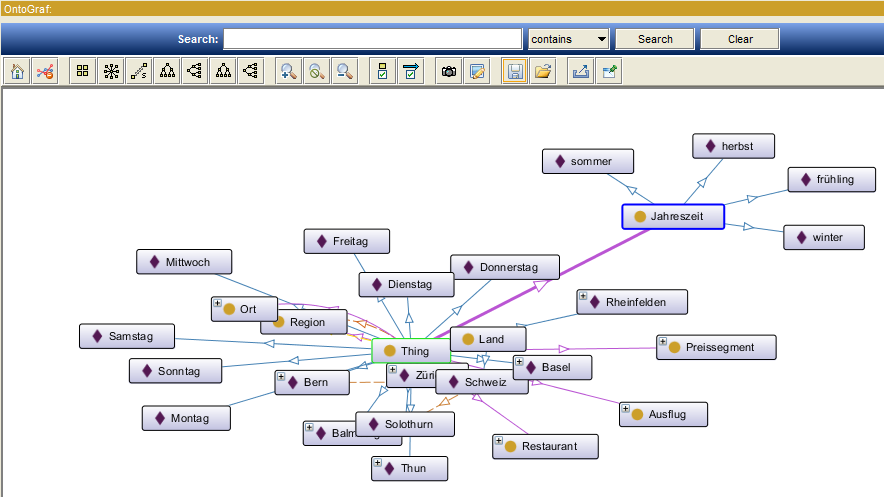
\includegraphics[scale=0.7]{bilder/OntoGraf.png}
    \caption{Beispiel der OntoGraf-Ansicht.\label{fig:kompo:ontograf}\protect\footnotemark}
\end{figure}
\footnotetext{Eigene Darstellung mittels Protégé.}

Schlussfolgerungen werden in allen Ansichten direkt zur Laufzeit des Reasoners bei allen Elementtypen ergänzt.

(vgl.~\cite{protegeView})

\section{Clark \& Parsia Stardog}
\label{sec:komponenten_stardog}
Bei Stardog handelt es sich um eine Graphdatenbank mit Unterstüztung des RDF-Graphenmodelles. Sie bietet den Import und Export von Ontologien in diversen Format an und die Möglichkeit Informationen einer Ontologie mittels SPARQL abzufragen. Des Weiteren unterstützt Stardog die Sprache OWL sowie SWRL-Regeln.\\
Pellet, in Stardog enthalten, bildet eine zentrale Komponente für die Schlussfolgerung.

Stardog bietet viele Kommunikationsschnittstellen, so z.B. HTTP und SNARL.\\
Programmierschnittstellen sind für zahlreiche Sprachen, so beispielsweise Java, JavaScript oder Python vorhanden.

Stardog unterscheidet drei Versionen der Lizenzierung: Community, Developer und Enterprise. Die Versionen unterscheiden sich durch maximale Anzahl der verwaltbaren Datenbanken und der möglichen Tripel pro Datenbank, Anzahl gleichzeitiger Verbindungen und durch Anzahl Benutzer und Rollen. Je nach gewählter Lizenzierung leistet der Hersteller eine Kundenbetreuung.

(vgl.~\cite{stardogDocu})

\subsection{Reasoner}
\label{subsec:komponenten_reasoner}
Reasoner sind Komponenten,  die Folgerungen von implizitem Wissen zulassen bzw.\ anbieten. Es handelt es sich um eine Art ``Verstehen'' der Maschinen. Ziel ist es, aus explizitem Wissen in Form einer Ontologie implizites Wissen zu gewinnen.

Wie bereits unter~\autoref{ssubsec:vorgehen:grundlagen:technisch} erwähnt, wurde Pellet als Reasoner (Anwendung zum Ziehen von Schlüssen) gewählt. Eine detaillierte Beschreibung von Pellet findet sich im~\hyperref[sec:anhang:tutorial_dokument]{Tutorial} unter Abschnitt 6.4.

\subsection{Konkrete Anwendung der Komponenten zur Modellierung der Ontologie}
\label{subsec:komponenten_anwendung}
Im Laufe der Arbeit hat sich herausgestellt, dass das Schlussfolgern in Protégé nicht einwandfrei funktioniert. Gewisse SPARQL-Anfragen wurden nicht erwartungsgemäss beantwortet.

Da sowohl Protégé als auch Stardog dieselbe Komponente für Schlussfolgerungen (den Pellet-Reasoner) verwenden, muss es sich bei dem Fehlverhalten um einen Fehler bei der Aufbereitung der Abfragen handeln.

In Protégé existiert zudem keine HTTP-Schnittstelle. Es existiert zwar eine Programmierschnittstelle mit welcher eine HTTP-Schnittstelle geschaffen werden kann. Dies wurde aus zeitlichen Gründen verworfen.

Angesichts der Funktionsstörung und mangelnder HTTP-Schnittstelle, wurde die Ontologie in Protégé erstellt und bearbeitet. Die Weiterverarbeitung der Ontolgie erfolgte mittels Stardog, da Stardog die SPARQL-Anfragen korrekt beantwortet und ausserdem eine HTTP- und REST-Schnittstelle bietet.

Dafür musste in Stardog eine neue Datenbank erstellt werden. In diese wurde die mittels Protégé vorbereitete Ontologie im RDF/XML-Format eingespielt.

Stardog bietet bei der Verwendung des Reasoners mehr Möglichkeiten als die anderen Werkzeuge (wie zum Beispiel Protégé). Schlussfolgerungen mittels einer Kombination von RDFS-, QL-, RL- und EL-Axiomen sowie zusätzlich SWRL-Regeln gezogen werden. Details finden sich unter~\footnote{\url{http://docs.stardog.com/\#_reasoning_levels}}.


Durch die Kombination dieser beiden Werkzeuge Protégé und Stardog konnte eine zuverlässige Modellierung und Verwendung der Ontologie erreicht werden.

\section{Benuzteroberfläche}
\label{sec:komponenten:ember}
Ein Teil der Aufgabe bestand darin, eine möglichst benutzerfreundliche Schnittstelle zwischen Mensch und System zu entwickeln.\\
Als Schnittstelle haben die Autoren eine Webapplikation zur Reiseplanung entwickelt, wie im~\autoref{sec:loesung_gui} ausgeführt. Diese ermöglicht das Planen einer Reise mit Hilfe eines Assistenten. Der Benutzer kann die gewünschten Reisekriterien auswählen und erhält schliesslich eine Auswahl an Reiseobjekten, welche seinen Kriterien entsprechen.

\subsection{Komponenten der Benutzeroberfläche}
\label{subsec:komponenten:gui:komponenten}
Folgende Komponenten wurden zur Umsetzung der Benutzeroberfläche gewählt:
\begin{itemize}
    \item \textit{Vagrant}\footnote{\url{http://www.vagrantup.com}}\\
        Virtualisierungslösung
    \item \textit{nginx}\footnote{\url{https://nginx.org}}\\
        Webserver
    \item \textit{Ember.js}\footnote{\url{http://emberjs.com}}\\
        Applikations-Framework
    \item \textit{Bootstrap}\footnote{\url{http://getbootstrap.com}}\\
        HTML-, CSS- und JavaScript-Framwork von Twitter
\end{itemize}
(Die Auswahl erfolgte aufgrund beruflicher Erfahrungen der Autoren.)

\subsubsection{Vagrant}
\label{ssubsec:komponenten:gui:komponenten:vagrant}
Bei Vagrant handelt es sich um ein Werkzeug zur Erstellung von vollständigen Entwicklungsumgebungen basierend auf Virtualisierung (vgl.~\cite{vagrant}). Details dazu finden sich unter~\footnote{http://www.vagrantup.com/about.html}.

In der vorliegend Arbeit wurde Vagrant zur Bereitstellung einer (virtuellen) Entwicklungsumgebung genutzt. Dabei wird die eigentliche Anwendung von der Entwicklungsumgebung getrennt. Dadurch kann die Entwicklungsumgebung jederzeit mittels weniger Befehle wieder neu aufgebaut werden.

\subsubsection{nginx}
\label{ssubsec:komponenten:gui:komponenten:nginx}
nginx (``engine x'' ausgesprochen) ist ein freier open-source Webserver. Seine Stärken liegen unter anderem  auf hoher Leistung, hoher Nebenläufigkeit und geringem Speicherverbrauch. Er ist der am zweithäufigsten eingesetzte Webserver (vgl.~\cite{nginx}).

nginx wurde innerhalb der (virtuellen) Entwicklungsumgebung zur Bereitstellung der Applikation genutzt. So kann die Applikation innerhalb eines Rechners wie eine externe Webseite angesprochen werden.

\subsubsection{Ember.js}
\label{ssubsec:komponenten:gui:komponenten:emberjs}
Ember.js ist ein clientseitiges open-source Framework zur Erstellung von Webapplikationen. Es baut auf dem Model-View-Controller (MVC) Softwarearchitektur-Muster auf. Es erlaubt die Erstellung von skalierbaren Anwendungen mittels einer einzigen Datei und bietet dabei deklarative Datenbindung, dynamische Eigenschaften, automatisch aktualisierte Templates sowie eine Zustandsverwaltung der Applikation mittels einer Router-Komponente (vgl.~\cite{ember}).

Ember.js wurde für die Umsetzung der Applikationslogik der Benutzeroberfläche eingesetzt.

\subsubsection{Bootstrap}
\label{ssubsec:komponenten:gui:komponenten:bootstrap}
Bootstrap der Firma Twitter ist eine Sammlung von Werkzeugen um Webseiten und Webapplikationen zu erstellen. Bootstrap bietet unter anderem verschiedene, auf HTML und CSS basierende Vorlagen für Typographie, Formulare, Schaltflächen und Navigation (vgl.~\cite{bootstrap}).

Bootstrap wurde zur grafischen Gestaltung der Benutzeroberfläche eingesetzt.

\subsection{Architektur}
\label{subsec:komponenten:gui:architektur}
\begin{figure}[H]
    \centering \rotatebox{0}{\scalebox{0.5}[0.5]{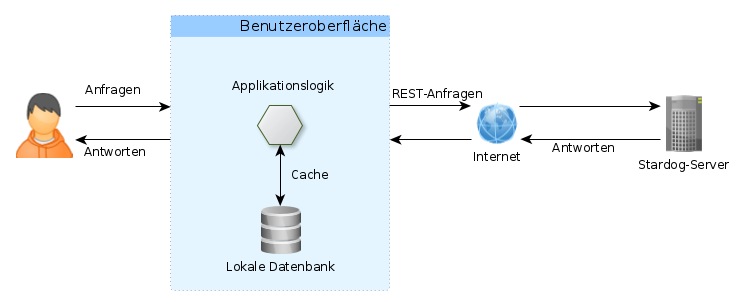
\includegraphics{bilder/architektur_gui.png}}}
    \caption{Architektur der Benutzeroberfläche\label{fig:architektur:gui}\protect\footnotemark}
\end{figure}
\footnotetext{Eigene Darstellung mittels yEd.}

Die obenstehende Abbildung~\ref{fig:architektur:gui} zeigt die Architektur der Benutzeroberfläche, bestehend aus einem Frontend und einem Backend. Mit Frontend ist die Applikation selbst (Benutzeroberfläche) gemeint, mit Backend der Stardog-Server.

Die Applikation besteht aus \textit{Modellen}, \textit{Ansichten} und \textit{Routen}.

\textit{Modelle} sind \textit{Reisen}, \textit{Dateneigenschaften} und \textit{Objektrelationen}.\\
\hangindent=1.5cm Das \textit{Modell} \textit{Reise} entspricht \textit{Individuen}, das \textit{Modell} \textit{Dateneigenschaft} \textit{DataProperties} und\\
das \textit{Modell} \textit{Objektrelation} den \textit{ObjectProperties} der Ontologie.

\textit{Routen} definieren, entsprechend ihrem Namen, den Ablauf der Applikation.\\
\hangindent=1.5cm \textit{Welcome}-Route ist der Einstieg der Applikation. Von der \textit{Welcome}-Route aus werden die \textit{Routen} \textit{Step1}, \textit{Step2} und \textit{Step3} nacheinander in Form eines Schritt-für-Schritt-Assistenten durchlaufen.\\
In Schritt 1 wird die Art der Ausflüge gewählt.\\
In Schritt 2 werden die \textit{Dateneigenschaften} sowie die \textit{Objektrelationen} pro zuvor gewählter Art der Ausflüge gewählt.\\
Schritt 3 gibt alle Instanzen zurück, welche den gewählten Kriterien entsprechen.\\
\\
Da in Schritt 1 nur bestimmte Individuen der Ontologie angezeigt werden sollen, wurden in der Ontologie diese Individuen mit der \textit{Dateneigenschaft} ``reise'' gekennzeichnet. Dadurch beschränkt sich die Abfrage von Schritt 1 nur auf diese Individuen.

Die \textit{Ansichten} kombinieren die Gestaltung (das Layout) der Seite mit der Ansicht der aktuellen Route.

Die gewählte Graphdatenbank Stardog bietet externen Zugriff via REST-Protokoll. Das gewählte Framework Ember.js bietet REST-Unterstützung via REST-Adapter an. Der REST-Adapter implementiert standardmässig Lesen und Schreiben einer REST-Schnittstelle.

Da das Ziel der Arbeit nicht eine vollständige Umsetzung (Lesen und Schreiben) der Ontologie war, wurde der Zugriff auf die Datenbank nur lesend implementiert. Dadurch kann die umgesetzte Applikation und somit der Benutzer Daten der Ontologie nur lesen (und nicht ändern). Daher musste das Standardverhalten des REST-Adapters von Ember.js durch Nutzung der lokalen Datenbank von Ember.js umgangen werden.

Beim initialen Aufruf der Applikation wird die gesamte Ontologie via REST-Protokoll vom Server abgerufen und nur in der lokalen Datenbank von Ember.js in Form der \textit{Modelle} abgelegt. Damit der Benutzer beim initialen Aufruf der Applikation nicht auf den Datenaustausch warten muss und die Applikation nicht blockiert wird, findet der Datenaustausch asynchron statt. Trotz im  Hintergrund laufender Anfragen kann die Applikation benützt werden. Dabei werden die \textit{Modelle} an die \textit{Ansicht} gebunden. Das heisst, erhält die Applikation Daten eines Modells, wird automatisch dessen \textit{Ansicht} dargestellt bzw.\ aktualisiert.

\chapter{Fazit und Ausblick}
\label{chap:fazit}

% In diesem Kapitel legen Sie Ihre kritische Betrachtung Ihrer Arbeit dar. Zeigen Sie, was Sie erreicht haben. Hinterfragen Sie das Ergebnis auf objektive Art und Weise.

Im Kapitel Lösung wurde bereits festgestellt, dass sämtliche Ziele der Arbeit erreicht wurden. Dabei ist wichtig, dass wir im Laufe der Arbeit die Problemdomäne ändern geändert haben. Die ursprünglich gewählte Domäne des Erlernens des Programmierens anhand der Programmiersprache Prolog stellte sich als nicht geeignet heraus.

Als wir dieses Gebiet auswählten, wussten wir noch zu wenig über die Wissensmodellierung mittels Ontologien. So war uns nicht bewusst, dass sich diese vor allem für solche Gebiete eignet, in denen viele Fakten vorhanden sind. Das Erlernen des Programmierens anhand Prolog ist ein sehr theoretisches Gebiet mit Abläufen und Verallgemeinerungen. Im Gegensatz ist die das Planen von Reisen viel besser dazu geeignet. Damit war es uns möglich die verschiedenen Spezialitäten eines Expertensystems herauszufinden und die Mächtigkeit von semantischen Datenbanken aufzuzeigen.

Bei unserer Arbeit lag der Fokus nicht auf einem genau definierten Endprodukt. Viel mehr stand der gesamte Prozess der Wissenserarbeitung im Vordergrund. Ein wichtiger Teil war die Modellierung einer Ontologie. Hierbei war es schwierig ein sinnvolles, allgemeines Vorgehen zu finden und definieren. So sehen wir die verschiedenen Schwierigkeiten, auf welche wir während des Prozesses gestossen sind, nicht als Nachteil sondern als Erfahrung an.

Wir haben uns bewusst für ein für uns eher unbekanntes Thema der Thesis entschieden. Dies vor allem, weil wir in der Erarbeitung der Bachelor Thesis eine Chance sahen zu forschen und zu experimentieren. In der Berufswelt, welche jetzt auf uns wartet wird dies wahrscheinlich nur noch begrenzt möglich sein. Uns ist aber erst beim Reflektieren der Arbeit richtiggehend bewusst geworden, dass wir ein Themengebiet gewählt haben bei dem wir ausser einigen simplen Grundlagen alles neu erarbeiten mussten. Es war uns nur sehr bedingt möglich, vorhandenes Wissen anzuwenden. Dies führte zu einer sehr spannenden und intensiven Arbeit.

Als Vorbereitung für die Bachelor Thesis besuchten wir das Wahlpflichtfach Künstliche Intelligenz. In diesem Modul, hatten wir die Möglichkeit uns zumindest oberflächlich mit der Programmiersprache Prolog auseinander zusetzten. Aus diesem Grund entstanden regelmässige Vergleiche zwischen Expertensystemen welche auf Ontologien aufbauen und Prolog. Ein eindeutiger Vorteil von Wissensmodellierung auf Basis von Ontologien mittels OWL ist, dass es einige Werkzeuge gibt, welche die Modellierung unterstützten. So können mithilfe von Protégé auf eine übersichtliche Art Fakten abgebildet werden. Dies wird noch unterstützt durch die Tatsache, dass in OWL eine klare Klassen - Eigenschaft - Beziehungstrennung bestet. Dies führt zu einem Raster welches zu einer verbesserten Trennung führt. Die XML ähnliche Syntax ermöglicht zudem eine\\ 

%- Wissensmodellierung hat vor und nachteile:\\
%   Vorteile: html schnittstelle; mit vorhandenen Werkzeugen wird es übersichtlicher (Protege)\\
%   Nachteile: Regeln mit Indiviuen nicht möglicht; Rechnen nur eingeschränkt möglich\\
%- Struktur der ARbeit sinnvoll; mit erarbeiten der Grundlagen und Praktischer Umsetztung
%Vorteile und Nachteile
%+ Sehr klare Trennung Eigenschaften, Klassen und Relationen => klares Raster
%+ Verwendung von Logik / Ableitung von Regeln
%+ Mischform UML und Prolog
%- Abläufe sind sehr schwer abzubilden
%Ein grosser Vorteil im Vergleich zu anderen Expertensystemen ist sicher, dass die OWL / XML Schreibweise gut verarbeitet werden kann und es sich so anbietet HTML-Schnittstellen zu genieren und zu nutzen.  (TODO soll hier gesagt werden was?). 

% - Zusammenfassung des Resultats
% - Würdigung des Resultats
% - Evtl. Empfehlungen zum weiteren Vorgehen

\section{Ausblick}
\label{sec:fazit_subchap}
Bei dem aktuellen Modell der Ontologie sowie der Benutzeroberfläche handelt es sich um einen Nachweis der Machbarkeit in Form von Prototypen. Der Funktionsumfang dieser beschränkt sich daher nur auf das Nötigste und entspricht nicht einer realen Anwendung.

Wollte man das Umgesetzte einer praxisrelevanten Anwendung nutzen, so müsste dies erweitert werden. Die Ontologie verfügt nur über einige wenige, exemplarische Entitäten. Um interessante Abfragemöglichkeiten bieten zu können, wäre sicherlich eine starke Erweiterung der Ontologie nötig.

Weiter könnte die Anwendung mit Benutzerprofilen versehen werden, welche den Standort des Benutzers speichern. Mittels einer Geoinformationssoftware könnte so die Distanz zu Entitäten (z.B. Restaurants und Ausflüge) dynamisch berechnet werden.

Das Modell unterstützt aktuell nur eine Zeitauflösung von einem halben Tag, einem ganzen Tag sowie mehr als einem Tag. Eine feinere Zeitauflösung, etwa in Form von Fliesskommawerten, liesse eine genauere Planung von Reisen zu. Dies müsste jedoch in Form von Applikationslogik und nicht durch den Reasoner umgesetzt werden, da dieser, wie im Tutorial erwähnt, keine Bedingungserfüllungsprobleme lösen kann.



\chapter{Schlussbemerkung}
\label{chap:schlussbemerkung}

% Falls vorhanden, können Sie hier Ihren Dank ausprechen. Sie können hier auch Kommentare zum Umfeld der Arbeit abgeben, zum Beispiel über die Betreuung oder den Auftraggeber.

%---------------------------------------------------------------------------

% Selbständigkeitserklärung
%---------------------------------------------------------------------------
\cleardoublepage{}
\phantomsection{}
\addcontentsline{toc}{chapter}{Selbständigkeitserklärung}
\chapter*{Selbständigkeitserklärung}
\label{chap:selbstaendigkeitserklaerung}

\vspace*{10mm} 

Ich/wir bestätige/n, dass ich/wir die vorliegende Arbeit selbstständig und ohne Benutzung anderer als der im Literaturverzeichnis angegebenen Quellen und Hilfsmittel angefertigt habe/n. Sämtliche Textstellen, die nicht von mir/uns stammen, sind als Zitate gekennzeichnet und mit dem genauen Hinweis auf ihre Herkunft versehen. 

\vspace{15mm}

\begin{tabbing}
xxxxxxxxxxxxxxxxxxxxxxxxx\=xxxxxxxxxxxxxxxxxxxxxxxxxxxxxx\=xxxxxxxxxxxxxxxxxxxxxxxxxxxxxx\kill
Ort, Datum:		\> [Biel/Burgdorf], \versiondate \\ \\ 
Namen Vornamen:	\> [Test Peter] 	\> [Müster Rösä] \\ \\ \\ \\ 
Unterschriften:	\>......................................\>......................................\\
\end{tabbing}

%---------------------------------------------------------------------------

% Glossary
%---------------------------------------------------------------------------
%\cleardoublepage
\phantomsection{}
\addcontentsline{toc}{chapter}{Glossar}
\renewcommand{\glossaryname}{Glossar}
\printglossary{}
%---------------------------------------------------------------------------

% Bibliography
%---------------------------------------------------------------------------
%\cleardoublepage
%\phantomsection{}
%\addcontentsline{toc}{chapter}{Literaturverzeichnis}
%\bibliographystyle{unsrtdin}
\bibliographystyle{unsrtnat}
\bibliography{datenbanken/bibliography}{}
%---------------------------------------------------------------------------

% Listings
%---------------------------------------------------------------------------
%\cleardoublepage
\phantomsection{}
\addcontentsline{toc}{chapter}{Abbildungsverzeichnis}
\listoffigures
%\cleardoublepage
%\phantomsection{}
%\addcontentsline{toc}{chapter}{Tabellenverzeichnis}
%\listoftables
%---------------------------------------------------------------------------

% Index
%---------------------------------------------------------------------------
%\cleardoublepage
%\phantomsection{}
%\addcontentsline{toc}{chapter}{Stichwortverzeichnis}
%\renewcommand{\indexname}{Stichwortverzeichnis}
%\printindex
%---------------------------------------------------------------------------

% Attachment:
%---------------------------------------------------------------------------
\appendix
\settocdepth{section}
\begin{titlepage}


    \clearpage
    \vspace*{\fill}
    \begin{center}
        \begin{minipage}{.6\textwidth}
            \fontsize{26pt}{28pt}\selectfont
            Anhang
        \end{minipage}
    \end{center}
    \vfill % equivalent to \vspace{\fill}
    \clearpage


\end{titlepage}

\newpage 

% In den Anhang fügen Sie ein:
%  * Details des Projektpans, falls vorhanden
%  * Resultate und Zwischenresultate in Funktion der Projektiterationen
%  * Pflichtenheft / Anforderungsspezifikation (Stand Ende dritter Woche)
%  * Angaben zum Projektrepository
%  * Sitzungsprotokolle, falls vorhanden
%  * Weiterführende Erläuterungen zu den verwendeten Technologien, falls nötig
%  * Benutzerhandbuch, falls vorhanden und sinnvoll, es hier aufzulisten
%  * Installations- und Betriebsdokument, falls vorhanden und sinnvoll, es hier aufzulisten
% Unterlassen Sie das Anfügen von Listings.

\appendix

\section*{Anforderungen}
\label{sec:anhang:anforderungen}
\href{anhang/anforderungen.pdf}{Anforderungsdokument}

\section*{Beispiele}
\label{sec:anhang:sparql_beispiele}
\href{anhang/schnipsel.pdf}{Dokument mit diversen Abfragebeispielen}

\section*{Dokumentation Wissensmodellierung}
\label{sec:anhang:tutorial_dokument}
\href{../Tutorial/template.pdf}{Dokumentation Wissensmodellierung}

\section*{Dokumentation BTI7302 --- Projekt2}
\label{sec:anhang:projekt2}
\href{../Extern/EigeneDokumente/DokumentationProjekt2.pdf}{Dokumentation BTI7302 - Projekt2}

\section*{Arbeitsjournal}
\label{sec:anhang:journal}
TODO:\@ Journal hier einfügen.

\section*{Benuterhandbuch}
\label{sec:anhang:handbuch}
TODO:\@ Handbuch hier einfügen.

\section*{Grafiken}
\label{sec:anhang:grafiken}
TODO:\@ Grafiken hier einfügen.

\section*{Reiseplaner}
\label{sec:anhang:reiseplaner}
TODO:\@ Reiseplaner hier einfügen.

%---------------------------------------------------------------------------

%---------------------------------------------------------------------------
\end{document}
